\documentclass[12pt]{report}

%Packages-------------------------------------
\usepackage{amsmath}
\usepackage{amsfonts}
\usepackage{amssymb}
\usepackage{amsthm}
\usepackage{graphics}
\usepackage{graphicx}
\usepackage{subcaption}
\usepackage[colorlinks=true,
            linkcolor=blue,
            citecolor=blue,
            urlcolor=blue]{hyperref}
\usepackage{longtable}
%\usepackage{xtocnic}
\usepackage{float}
\usepackage{array}
\usepackage{caption}
\usepackage{tabularx} % Required for auto-fitting
\usepackage{booktabs} % For better looking lines
\usepackage{tikz}
\usetikzlibrary{positioning, arrows.meta}


\usepackage{xepersian}
\settextfont{XB Zar.TTF}
\settextfont[
  Path = ./, % or the folder where fonts are stored
  BoldFont = XB ZarBd.ttf
]{XB Zar.ttf}

\AtBeginDocument{\renewcommand{\bibname}{مراجع}}
%Layout---------------------------------------

%\usepackage[top=2cm, bottom=2cm, left=2cm, right=2cm]{geometry}

%Commands-------------------------------------


%Theorems-------------------------------------
\newtheorem{thm}{قضیه}[chapter]
\newtheorem{cor}[thm]{نتیجه}
\newtheorem{defn}[thm]{تعریف}
\newtheorem{prop}[thm]{گزاره}
\newtheorem{lmm}[thm]{لم}
\newtheorem{conj}[thm]{حدس}
\newtheorem{exm}[thm]{مثال}
\newtheorem{rem}[thm]{تذکر}
\newtheorem{note}[thm]{یادداشت}
\newtheorem{alg}[thm]{الگوریتم}

\setcounter{tocdepth}{3}



\begin{document}

%Title page ---------------------------------------------

\begin{figure}
\centering

\includegraphics[height=2.5cm]{UT-Logo.pdf}
\end{figure}

\begin{center}
پردیس علوم
\\
دانشکده ریاضی، آمار و علوم کامپیوتر
\end{center}

\begin{center}
%%%%%%%%%%%%%
\end{center}

\begin{center}
\huge{شناسايی فعالیت‌های گروهی برای تحلیل ویدیوهای ورزشی}
\end{center}

\begin{center}
%%%
\end{center}

\begin{center}
نگارنده
\end{center}
\begin{center}
\textbf{امید نائیج نژاد}
\end{center}

\begin{center}
\begin{tabular}{rr}
استاد راهنما: دکتر ضیائی تبار

\end{tabular}
\end{center}

\vspace{3cm}
\begin{center}
پایان‌نامه برای دریافت درجه کارشناسی
\\
در رشته علوم کامپیوتر
\end{center}

\begin{center}
خرداد 1405
\end{center}

\pagestyle{empty}
\pagenumbering{}

\newpage
%\pagestyle{headings}
%\setcounter{page}{1}
%\pagenumbering{roman}
\pagestyle{plain}
\setcounter{page}{1}
\pagenumbering{harfi}
%Abstract page-------------------------------
\chapter*{}
\section*{چکیده}
در سال‌های اخیر، تحلیل خودکار ویدیو و درک فعالیت‌های گروهی به یکی از مسائل مهم در حوزه بینایی ماشین تبدیل شده است. یکی از زیرشاخه‌های این حوزه، تشخیص فعالیت گروهی\LTRfootnote{Group Activity Recognition} است که هدف آن شناسایی رفتار جمعی افراد در یک صحنه بر اساس تعاملات فضایی و زمانی میان آن‌ها می‌باشد. این مسئله به‌ویژه در تحلیل ویدیوهای ورزشی اهمیت بالایی دارد، زیرا درک صحیح فعالیت‌های تیمی می‌تواند کاربردهای گسترده‌ای در تحلیل تاکتیکی، ارزیابی عملکرد و سیستم‌های هوشمند ورزشی داشته باشد.

هدف اصلی این پژوهش، بررسی و ارزیابی رویکردهای مبتنی بر یادگیری عمیق برای تشخیص فعالیت‌های گروهی در ویدیوهای ورزشی است. در این راستا، چندین معماری مختلف شامل مدل‌های مبتنی بر شبکه‌های عصبی کانولوشنی-بازگشتی و همچنین معماری‌های مبتنی بر ترنسفورمر مورد بررسی و پیاده‌سازی قرار گرفته‌اند تا توانایی هر یک در مدل‌سازی وابستگی‌های فضایی و زمانی در داده‌های ویدیویی تحلیل شود.

آزمایش‌ها بر روی مجموعه‌داده‌ای از ویدیوهای ورزشی انجام شده و عملکرد مدل‌ها با استفاده از معیارهای استاندارد ارزیابی مثل \lr{F1-score} سنجیده شده است. نتایج به‌دست‌آمده نشان می‌دهد که مدل‌های مبتنی بر ترنسفورمر، به‌ویژه در مدل‌سازی روابط بلندمدت زمانی، عملکرد رقابتی و در برخی موارد برتری نسبت به روش‌های سنتی‌تر دارند. با این حال، محدودیت‌هایی مانند اندازه کوچک داده‌ها و پیچیدگی محاسباتی همچنان تأثیر قابل توجهی بر عملکرد نهایی دارند.

در مجموع، این پژوهش ضمن ارائه یک مقایسه جامع میان رویکردهای مختلف، نشان می‌دهد که انتخاب معماری مناسب در مسئله تشخیص فعالیت گروهی باید با توجه به محدودیت داده و منابع محاسباتی انجام شود. این نتایج می‌تواند به عنوان پایه‌ای برای تحقیقات آینده در زمینه تحلیل ویدیوهای ورزشی و توسعه مدل‌های کارآمدتر مورد استفاده قرار گیرد.


%Dedication page-----------------------------
%\chapter*{تقدیم به}
%\section*{تقدیم به}

%Acknowledgement page------------------------
\chapter*{}
\section*{سپاسگزاری}
از استاد بزرگوارم سرکار خانم دکتر ضیایی تبار که با کمک‌ها و راهنمایي‌های بی‌دریغشان، نقش
به‌سزایی در پیشبرد این پروژه ایفا کردند، صمیمانه سپاسگزارم.

% \vspace{.5cm}

% همچنین از KAUST برای فراهم کردن دسترسی به دیتاست SoccerNet جهت استفاده‌های پژوهشی و آموزشی سپاسگزارم.% این دسترسی نقش مهمی در انجام این پایان‌نامه کارشناسی داشت.

%copyright + declaration page
%\chapter*{اصالت اثر}
%\section*{اصالت اثر}
% هیچ قسمت از این پایان‌نامه، پیش از این در هیج موسسه تحصیلات عالی برای دریافت درجه تحصیلی استفاده نشده است. همچنین، هیچ قسمت از این پایان‌نامه برگردان فارسی تمامی یا قسمتی از یک اثر دیگر علمی (مانند مقاله، پایان‌نامه، و غیره) به زبانی دیگر نمی‌باشد. ارائه این پایان‌نامه توسط نگارنده به معاونت آموزشی (معاونت پژوهشی و تحصیلات تکمیلی برای ارشد و دکتری) به منزله تعهد نگارنده به اصالت متن و محتوای ارائه شده بر اساس یک کار پژوهشی در مدت تحصیل در دانشگاه تهران می باشد. در صورت اثبات خلاف این امر، مدرک تحصیلی اخذ شده توسط این پایان‌نامه از دانشگاه تهران، معتبر نمی باشد. 
%
%\chapter*{حق مالکیت معنوی}
%\section*{حق مالکیت معنوی}
%حق مالکیت معنوی این اثر متعلق به دانشگاه تهران می باشد. استفاده از مطالب این پایان‌نامه در فعالیت‌های تحقیقاتی با ذکر منبع بلامانع می‌باشد. در صورت استفاده تجاری، مانند چاپ این پایان‌نامه، هماهنگی لازم و اجازه کتبی از دانشگاه و نگارنده پایان‌نامه الزامی می‌باشد.

%\listoffigures

%-------------------------
%\pagestyle{plain}
%\setcounter{page}{1}
%\pagenumbering{harfi}
%-------------------------


\chapter*{پیشگفتار}

مسئله تشخیص فعالیت‌های گروهی در ویدیوهای ورزشی یکی از موضوعات مهم و نسبتاً جدید در حوزه بینایی ماشین به شمار می‌رود که هدف آن، درک خودکار رفتار جمعی افراد در یک صحنه ویدئویی است. در این مسئله، برخلاف تحلیل تک‌فردی، سیستم باید بتواند روابط و تعاملات میان چندین فرد را به‌صورت هم‌زمان درک کرده و بر اساس آن، نوع فعالیت کلی گروه را تشخیص دهد. این موضوع به‌طور مستقیم با چالش‌هایی مانند تغییرات سریع حرکتی، هم‌پوشانی افراد، تنوع دید دوربین و پیچیدگی تعاملات انسانی همراه است.

تلاش برای حل این مسئله سابقه‌ای نسبتاً طولانی در حوزه بینایی ماشین دارد. در ابتدا، روش‌های مبتنی بر ویژگی‌های دستی و مدل‌های کلاسیک یادگیری ماشین مورد استفاده قرار می‌گرفتند که معمولاً توانایی محدودی در درک روابط پیچیده زمانی و مکانی داشتند. با پیشرفت یادگیری عمیق، به‌ویژه شبکه‌های کانولوشنی و سپس مدل‌های مبتنی بر توالی و ترنسفورمرها، رویکردهای جدیدی برای استخراج ویژگی‌های فضایی و زمانی معرفی شدند که توانستند عملکرد این حوزه را به‌طور قابل توجهی بهبود دهند. در میان این تلاش‌ها، مدل‌هایی مانند شبکه‌های سه‌بعدی کانولوشنی، شبکه‌های ترکیبی CNN-RNN و معماری‌های ترنسفورمری، نقش مهمی در توسعه روش‌های نوین تشخیص فعالیت گروهی ایفا کرده‌اند. از جمله کارهای مهم در این حوزه می‌توان به پژوهش‌های انجام‌شده بر روی مدل‌های ویدئویی مبتنی بر ترنسفورمر مانند TimeSformer و همچنین مدل‌های مبتنی بر توکن‌سازی ویدئو مانند ViT اشاره کرد که مسیر جدیدی را در تحلیل داده‌های ویدئویی باز کرده‌اند.

اهمیت این پژوهش در آن است که تشخیص دقیق فعالیت‌های گروهی، کاربردهای گسترده‌ای در تحلیل مسابقات ورزشی، سیستم‌های نظارت تصویری، تحلیل رفتار جمعی و حتی سیستم‌های هوشمند کمک‌داور دارد. از این رو، بهبود دقت و پایداری مدل‌ها در این حوزه می‌تواند تأثیر مستقیمی بر عملکرد سیستم‌های واقعی داشته باشد.

در این پایان‌نامه، مجموعه‌ای از مدل‌های یادگیری عمیق برای تشخیص فعالیت‌های گروهی مورد بررسی و مقایسه قرار گرفته‌اند. تمرکز اصلی بر تحلیل توانایی مدل‌ها در استخراج ویژگی‌های فضایی و زمانی از ویدیوهای ورزشی بوده است. در این راستا، مدل‌های مبتنی بر شبکه‌های کانولوشنی-بازگشتی و معماری‌های مبتنی بر ترنسفورمر مورد استفاده قرار گرفته‌اند و عملکرد آن‌ها در شرایط یکسان ارزیابی شده است.

ساختار پایان‌نامه به این صورت است که ابتدا در فصل اول، کلیات مسئله، اهمیت آن و زمینه‌های کاربردی تشخیص فعالیت گروهی ارائه می‌شود. در فصل دوم، پیشینه تحقیق و روش‌های موجود در این حوزه مورد بررسی قرار می‌گیرد. فصل سوم به معرفی داده‌ها و روش پیشنهادی اختصاص دارد و در آن فرآیند آماده‌سازی داده‌ها و پیاده‌سازی مدل‌ها توضیح داده می‌شود. در فصل چهارم، نتایج تجربی و تحلیل عملکرد مدل‌ها ارائه می‌گردد و در نهایت، فصل پنجم شامل جمع‌بندی نتایج و ارائه پیشنهادهایی برای کارهای آینده خواهد بود.

\tableofcontents
\newpage % Ensures the list starts on a new page

\listoftables
\newpage

\listoffigures
\newpage

%---------------------
\pagestyle{plain}
\setcounter{page}{1}
\pagenumbering{arabic}
%---------------------


\chapter{مقدمه}
\section{زمینه و پیشینه مسئله}
تشخیص فعالیت‌های گروهی \LTRfootnote{Group Activity Recognition (GAR)} یکی از مسائل بنیادین در حوزه بینایی ماشین\LTRfootnote{Machine Vision} است که هدف آن درک رفتار جمعی افراد در یک صحنه ویدئویی می‌باشد. برخلاف تشخیص کنش‌های فردی که تنها بر حرکات یک شخص تمرکز دارد، در GAR تعاملات میان چندین عامل (انسان‌ها) و همچنین ارتباط آن‌ها با زمینه محیطی اهمیت اساسی پیدا می‌کند.

از دیدگاه تاریخی و فلسفی، مسئله درک فعالیت‌های گروهی ریشه در تلاش برای پاسخ به این پرسش دارد که «چگونه می‌توان از رفتارهای فردی به درک رفتار جمعی رسید؟». در رویکردهای اولیه بینایی ماشین، تمرکز عمدتاً بر استخراج ویژگی‌های سطح پایین نظیر حرکت، لبه‌ها و مسیرهای حرکتی بود. این رویکردها بر این فرض استوار بودند که با ترکیب ویژگی‌های فردی می‌توان به یک نمایش مناسب از رفتار گروهی دست یافت. با این حال، این دیدگاه اغلب از مدل‌سازی تعاملات پیچیده و وابستگی‌های زمانی-مکانی بین افراد ناتوان بود.

با پیشرفت روش‌های یادگیری ماشین\LTRfootnote{Machine Learning}، به‌ویژه مدل‌های احتمالاتی مانند \lr{HMM\LTRfootnote{Hidden Markov Models (HMMs)}} و \lr{CRF\LTRfootnote{Conditional Random Fields (CRFs)}}، تلاش شد تا وابستگی‌های زمانی بهتر مدل‌سازی شوند. اما نقطه عطف اصلی در این حوزه با ظهور یادگیری عمیق\LTRfootnote{Deep Learning} رقم خورد. شبکه‌های عصبی کانولوشنی\LTRfootnote{Convolutional Neural Networks (CNNs)} امکان استخراج خودکار ویژگی‌های فضایی را فراهم کردند و مدل‌های بازگشتی\LTRfootnote{Recurrent Neural Networks (RNNs)} و بعدتر ترنسفورمرها\LTRfootnote{Transformers}، وابستگی‌های زمانی و تعاملات پیچیده‌تر را پوشش دادند. در سال‌های اخیر، استفاده از گراف‌ها و مکانیزم‌های توجه\LTRfootnote{Attention Mechanisms} برای مدل‌سازی روابط بین افراد، به یکی از جریان‌های اصلی پژوهشی در تشخیص فعالیت‌های گروهی تبدیل شده است.

به‌طور کلی، تحول تشخیص فعالیت‌های گروهی را می‌توان به گذار از «ویژگی‌های دست‌ساخته\LTRfootnote{Handcrafted Features}» به «یادگیری نمایش» و سپس به «مدل‌سازی تعاملات پیچیده» تعبیر کرد؛ گذاری که نشان‌دهنده حرکت این حوزه به سمت درک معنایی عمیق‌تر از صحنه‌های اجتماعی است.

\section{کاربردها}
\subsection{تحلیل ویدیوهای ورزشی}
یکی از مهم‌ترین حوزه‌های کاربردی تشخیص فعالیت‌های گروهی، تحلیل ویدیوهای ورزشی است. در ورزش‌هایی مانند فوتبال، بسکتبال و والیبال، بسیاری از رویدادهای کلیدی ماهیتی گروهی دارند و تنها با در نظر گرفتن تعاملات میان بازیکنان قابل درک هستند. به‌عنوان مثال، تشخیص موقعیت‌های گل، آرایش‌های تیمی، الگوهای پاس‌کاری و یا رفتارهای دفاعی، نیازمند تحلیل هم‌زمان چندین بازیکن و روابط میان آن‌ها است. استفاده از GAR در این حوزه می‌تواند به تحلیل تاکتیکی تیم‌ها، بهبود تصمیم‌گیری مربیان، داوری خودکار و تولید خلاصه‌های هوشمند از مسابقات منجر شود.

\subsection{نظارت و امنیت}
در سیستم‌های نظارتی، درک رفتارهای گروهی نقش مهمی در شناسایی موقعیت‌های غیرعادی دارد. فعالیت‌هایی مانند درگیری، تجمع‌های غیرمعمول یا رفتارهای تهدیدآمیز اغلب به‌صورت گروهی رخ می‌دهند و تشخیص آن‌ها نیازمند تحلیل تعاملات میان افراد است. GAR می‌تواند به‌عنوان یک ابزار کلیدی در افزایش امنیت محیط‌های عمومی مانند فرودگاه‌ها، ایستگاه‌های مترو، قطار و فضاهای شهری مورد استفاده قرار گیرد.

\subsection{حمل‌ونقل هوشمند}
در حوزه حمل‌ونقل، تحلیل رفتار جمعی عابران پیاده و وسایل نقلیه اهمیت زیادی دارد. درک نحوه حرکت گروهی افراد در تقاطع‌ها یا رفتار جمعی خودروها در شرایط مختلف ترافیکی می‌تواند به طراحی سیستم‌های هوشمندتر برای مدیریت ترافیک و افزایش ایمنی کمک کند. در این زمینه، GAR می‌تواند نقش مهمی در پیش‌بینی رفتارهای جمعی و جلوگیری از حوادث ایفا کند.

\subsection[رباتیک و تعامل انسان-ماشین]{رباتیک و تعامل انسان-ماشین\LTRfootnote{Human-Machine Interaction}}
در محیط‌های اجتماعی، ربات‌ها برای تعامل مؤثر با انسان‌ها نیازمند درک رفتارهای گروهی هستند. به‌عنوان مثال، یک ربات خدماتی باید بتواند رفتار یک گروه از افراد را تحلیل کرده و تصمیم‌گیری مناسبی انجام دهد. این مسئله به‌ویژه در محیط‌های شلوغ مانند مراکز خرید یا فرودگاه‌ها اهمیت پیدا می‌کند.

\subsection{تحلیل رفتار اجتماعی و سلامت}
درک رفتارهای گروهی می‌تواند در تحلیل الگوهای اجتماعی و حتی مسائل مرتبط با سلامت روان مورد استفاده قرار گیرد. بررسی نحوه تعامل افراد در محیط‌های اجتماعی می‌تواند به شناسایی الگوهای رفتاری خاص و حتی نشانه‌های اختلالات اجتماعی کمک کند. این کاربرد نشان‌دهنده اهمیت GAR فراتر از حوزه‌های فنی و در ارتباط با علوم انسانی است.

\section{تعریف مسئله}
مسئله تشخیص فعالیت‌های گروهی را می‌توان به‌صورت رسمی\LTRfootnote{Formal} به‌عنوان نگاشت\LTRfootnote{Mapping} یک دنباله ویدئویی به یک یا چند برچسب فعالیت تعریف کرد. فرض کنید یک ویدیو به‌صورت دنباله‌ای از فریم‌ها نمایش داده شود:

\[
V = \{I_1, I_2, \dots, I_T\}
\]

که در آن $T$ تعداد فریم‌ها است. در هر فریم، مجموعه‌ای از افراد حضور دارند که می‌توان آن‌ها را به‌صورت زیر نمایش داد:

\[
P_t = \{p_1, p_2, \dots, p_{N_t}\}
\]

در اینجا $N_t$ تعداد افراد در فریم $t$ است. هدف، یادگیری تابعی است که بتواند این دنباله ویدئویی را به یک برچسب فعالیت گروهی نگاشت کند:

\[
f: V \rightarrow Y
\]

که در آن $Y$ نشان‌دهنده کلاس فعالیت گروهی است. در تنظیمات پیچیده‌تر، این نگاشت می‌تواند به‌صورت تابعی از دنباله‌ای از برچسب‌ها در طول زمان یا حتی ترکیبی از برچسب‌های فردی و گروهی تعریف شود. این تعریف نشان می‌دهد که مسئله تشخیص فعالیت‌های گروهی، ذاتاً یک مسئله چندسطحی است که شامل تحلیل هم‌زمان اطلاعات فضایی، زمانی و رابطه‌ای می‌باشد.

\section{ابعاد و چالش‌ها}
یکی از مهم‌ترین ابعاد مسئله تشخیص فعالیت‌های گروهی، نیاز به مدل‌سازی تعاملات میان افراد است. رفتار گروهی تنها از طریق تحلیل مستقل هر فرد قابل درک نیست، بلکه روابط میان افراد نقش تعیین‌کننده‌ای دارند. این موضوع باعث می‌شود که مدل‌سازی وابستگی‌های بین‌فردی به یکی از چالش‌های اصلی تبدیل شود.

علاوه بر این، فعالیت‌های گروهی معمولاً در طول زمان شکل می‌گیرند و وابستگی‌های زمانی نقش مهمی در تعریف آن‌ها دارند. بنابراین، مدل باید قادر به درک پویایی‌های زمانی و ارتباط میان فریم‌های مختلف باشد. این مسئله به‌ویژه در سناریوهایی که فعالیت‌ها دارای ساختار زمانی پیچیده هستند، اهمیت بیشتری پیدا می‌کند.

تنوع در شرایط تصویربرداری نیز یکی دیگر از چالش‌های مهم است. تغییر در زاویه دید، نور، پس‌زمینه و تعداد افراد حاضر در صحنه می‌تواند باعث کاهش دقت مدل شود. همچنین، در بسیاری از مجموعه‌داده‌ها، توزیع کلاس‌ها نامتوازن است که این موضوع فرآیند یادگیری را با دشواری مواجه می‌کند.

در نهایت، افزایش تعداد افراد در صحنه منجر به رشد نمایی پیچیدگی در مدل‌سازی تعاملات می‌شود. این مسئله نیازمند طراحی مدل‌هایی است که بتوانند به‌صورت کارآمد و مقیاس‌پذیر این روابط را مدیریت کنند.

\section{اهمیت مسئله}
اهمیت تشخیص فعالیت‌های گروهی را می‌توان از چندین منظر مورد بررسی قرار داد. از منظر علمی، این مسئله در تقاطع بینایی ماشین، یادگیری ماشین و علوم شناختی قرار دارد و به درک بهتر رفتارهای اجتماعی کمک می‌کند. از منظر کاربردی، گستردگی کاربردهای آن در حوزه‌هایی مانند ورزش، امنیت، حمل‌ونقل و سلامت، نشان‌دهنده نقش حیاتی آن در سیستم‌های هوشمند مدرن است.

از منظر فنی نیز، GAR یکی از مسائل چالش‌برانگیز محسوب می‌شود که نیازمند ترکیب روش‌های پیشرفته در مدل‌سازی فضایی، زمانی و رابطه‌ای است. حل این مسئله می‌تواند به پیشرفت در سایر حوزه‌های مرتبط نیز منجر شود.

\section{سهم این پژوهش}
در این پایان‌نامه، تمرکز اصلی بر تشخیص فعالیت‌های گروهی در ویدیوهای ورزشی است. در این راستا، یک چارچوب مبتنی بر یادگیری عمیق برای تحلیل این نوع فعالیت‌ها ارائه می‌شود که قادر است ویژگی‌های فضایی و زمانی را به‌صورت مؤثر استخراج و ترکیب کند. همچنین، تلاش شده است تا با بررسی و مقایسه رویکردهای موجود، نقاط قوت و ضعف آن‌ها تحلیل شده و در طراحی مدل پیشنهادی مورد توجه قرار گیرد.

مدل ارائه‌شده در این تحقیق به‌گونه‌ای طراحی شده است که بتواند تعاملات میان افراد را به‌صورت کارآمد مدل‌سازی کند و در عین حال با چالش‌هایی مانند عدم توازن داده‌ها مقابله نماید. ارزیابی این مدل بر روی یک مجموعه‌داده واقعی انجام شده و نتایج حاصل، کارایی آن را در مقایسه با روش‌های موجود نشان می‌دهد.

\section{ساختار و نقشه راه}این پایان‌نامه در پنج فصل سازمان‌دهی شده است. در فصل دوم، مروری جامع بر ادبیات موضوع ارائه شده و رویکردهای مختلف در تشخیص فعالیت‌های گروهی مورد بررسی قرار می‌گیرند. فصل سوم به معرفی روش پیشنهادی اختصاص دارد و شامل تعریف دقیق مسئله، معماری مدل و جزئیات پیاده‌سازی است. در فصل چهارم، نتایج آزمایش‌ها و ارزیابی عملکرد مدل ارائه و تحلیل می‌شود. در نهایت، فصل پنجم به جمع‌بندی مطالب، نتیجه‌گیری و ارائه پیشنهاداتی برای پژوهش‌های آینده اختصاص دارد.

\chapter{مروری بر روش‌های پیشین}
\section{مقدمه}
تشخیص فعالیت گروهی یکی از زیرشاخه‌های بینایی کامپیوتر\LTRfootnote{Computer Vision} است که بر شناسایی رفتارهای جمعی انجام‌شده توسط چندین فرد در توالی‌های ویدیویی\LTRfootnote{Video Sequence} تمرکز دارد. برخلاف تشخیص کنش تک‌نفره\LTRfootnote{Single-person Action Recognition} که به دسته‌بندی اعمال مجزا می‌پردازد، در این حوزه لازم است روابط و تعاملات فضایی-زمانی\LTRfootnote{Spatio-temporal Relationships} میان چندین بازیگر مدل‌سازی شود تا بتوان یک فعالیت گروهی واحد را استنتاج کرد \cite{one,two}. این تفاوت بنیادی موجب شده است که تشخیص فعالیت گروهی به مسئله‌ای پیچیده‌تر و چندلایه‌تر نسبت به تشخیص کنش فردی تبدیل شود.

اهمیت این مسئله به‌ویژه در تحلیل ویدیوهای ورزشی\LTRfootnote{Sports Video Analysis} برجسته می‌شود، جایی که درک رفتارهای هماهنگ تیمی\LTRfootnote{Team Behavior}—مانند حملات سازمان‌یافته در بسکتبال، آرایش‌های دفاعی در فوتبال، یا استراتژی‌های تهاجمی در والیبال—نقش کلیدی در استخراج بینش‌های تاکتیکی و ارزیابی عملکرد دارد \cite{three,four}. در چنین سناریوهایی، تحلیل صرف رفتار فردی کافی نیست و لازم است تعاملات میان بازیکنان و ساختار کلی تیم نیز مورد توجه قرار گیرد.

با این حال، پیچیدگی‌های ذاتی این مسئله، از جمله انسداد\LTRfootnote{Occlusion}، تعاملات پویا میان بازیکنان، و نیاز به یکپارچه‌سازی اطلاعات در سطوح مختلف، چالش‌های قابل توجهی را ایجاد می‌کند. این عوامل باعث می‌شوند که مدل‌سازی دقیق روابط میان افراد و درک زمینه کلی صحنه از اهمیت ویژه‌ای برخوردار باشد \cite{three,five}. در این فصل، سیر تکامل روش‌های تشخیص فعالیت گروهی از رویکردهای اولیه مبتنی بر ویژگی‌های دست‌ساخته تا تکنیک‌های مدرن یادگیری عمیق بررسی شده و تمرکز ویژه‌ای بر کاربردهای ورزشی این حوزه خواهد بود.


\section{تکامل تشخیص فعالیت}
پژوهش در حوزه تشخیص فعالیت به‌صورت تدریجی و همگام با افزایش پیچیدگی سناریوهای مورد بررسی تکامل یافته است. در مراحل اولیه، تمرکز عمدتاً بر تشخیص کنش تک‌نفره\LTRfootnote{Single-person Action Recognition} بود، که هدف آن شناسایی اعمالی مانند دویدن یا پریدن در سطح فردی است \cite{six}. این رویکردها اگرچه در محیط‌های ساده عملکرد مناسبی داشتند، اما در مواجهه با تعاملات انسانی محدودیت‌هایی از خود نشان دادند.

در گام بعدی، توجه پژوهشگران به سمت تشخیص تعامل دو‌نفره\LTRfootnote{Two-person Interaction Recognition} معطوف شد، جایی که هدف مدل‌سازی روابط میان جفتی از افراد بود \cite{seven}. این سطح از تحلیل امکان درک ابتدایی از تعاملات انسانی را فراهم کرد، اما همچنان برای سناریوهای پیچیده‌تر کافی نبود.

در نهایت، تشخیص فعالیت گروهی به‌عنوان سطحی پیشرفته‌تر معرفی شد که در آن رفتارهای هماهنگ میان چندین فرد به‌صورت همزمان مورد تحلیل قرار می‌گیرد \cite{three}. این سطح از پیچیدگی مستلزم درک همزمان کنش‌های فردی و نحوه ارتباط آن‌ها در یک زمینه مشترک است. در کاربردهای ورزشی، این موضوع به معنای تحلیل ساختارهای تیمی، هماهنگی میان بازیکنان و تغییرات دینامیک در طول زمان است \cite{three,five}.


\section{روش‌های سنتی (پیش از یادگیری عمیق)}
پیش از ظهور یادگیری عمیق، رویکردهای تشخیص فعالیت گروهی عمدتاً بر ویژگی‌های دست‌ساخته و مدل‌های احتمالاتی ساخت‌یافته\LTRfootnote{structured probabilistic models} متکی بودند \cite{eight,nine}. این روش‌ها تلاش می‌کردند با طراحی ویژگی‌های مناسب و استفاده از مدل‌های آماری، رفتارهای گروهی را توصیف کنند.

در این چارچوب، ویژگی‌های فضایی-زمانی به‌صورت دستی استخراج می‌شدند. برای مثال، جریان نوری و مسیرهای حرکتی\LTRfootnote{Optical Flow and Motion Trajectories} به‌منظور توصیف حرکت، توصیف‌گرهای ظاهری\LTRfootnote{Appearance Descriptors} برای نمایش ویژگی‌های بصری، و روابط فضایی میان افراد\LTRfootnote{Spatial Relationships Between Individuals} برای درک ساختار صحنه مورد استفاده قرار می‌گرفتند. این ویژگی‌ها اگرچه قادر به ثبت برخی الگوهای حرکتی بودند، اما به دلیل ماهیت دستی خود، محدودیت‌هایی در پوشش تمامی جنبه‌های تعاملات پیچیده داشتند \cite{eight}.

برای مدل‌سازی پویایی‌های زمانی و وابستگی‌های میان افراد، از مدل‌های آماری ساخت‌یافته‌ای مانند مدل‌های مارکوف پنهان\LTRfootnote{Hidden Markov Models (HMMs)}، میدان‌های تصادفی شرطی\LTRfootnote{Conditional Random Fields (CRFs)} و میدان‌های تصادفی سلسله‌مراتبی\LTRfootnote{Hierarchical Random Fields} استفاده می‌شد. این مدل‌ها تلاش می‌کردند وابستگی میان کنش‌های فردی و فعالیت‌های گروهی را به‌صورت صریح نمایش دهند \cite{nine,ten}.

با وجود این تلاش‌ها، روش‌های سنتی با محدودیت‌های جدی مواجه بودند. وابستگی به ویژگی‌های دست‌ساخته باعث کاهش توان بازنمایی این مدل‌ها می‌شد و در نتیجه، عملکرد آن‌ها در صحنه‌های پیچیده با تعداد زیاد افراد کاهش می‌یافت. علاوه بر این، این روش‌ها در مدل‌سازی تعاملات پویا، به‌ویژه در محیط‌هایی مانند ورزش‌های تیمی، کارایی محدودی داشتند. این چالش‌ها در نهایت زمینه‌ساز حرکت به سمت رویکردهای مبتنی بر داده و یادگیری عمیق شدند \cite{three,four}.


\section{یادگیری عمیق برای تشخیص فعالیت گروهی}
ورود یادگیری عمیق نقطه عطفی اساسی در توسعه روش‌های تشخیص فعالیت گروهی محسوب می‌شود، زیرا این رویکرد امکان یادگیری خودکار بازنمایی‌های پیچیده و سلسله‌مراتبی را مستقیماً از داده فراهم می‌کند \cite{three,twelve}. برخلاف روش‌های سنتی که وابسته به طراحی دستی ویژگی‌ها بودند، مدل‌های یادگیری عمیق قادرند الگوهای پنهان در داده‌های بصری و زمانی را به‌صورت یکپارچه استخراج کنند. این ویژگی به‌ویژه در سناریوهای پیچیده مانند تحلیل ویدیوهای ورزشی، که شامل تعاملات چندگانه و تغییرات سریع صحنه است، اهمیت زیادی دارد.

\subsection{مدل‌های CNN-RNN و مدل‌های زمانی سلسله‌مراتبی}
در نخستین نسل از روش‌های مبتنی بر یادگیری عمیق، تلاش شد تا ویژگی‌های فضایی و زمانی به‌صورت مجزا اما مکمل مدل‌سازی شوند. در این چارچوب، شبکه‌های عصبی کانولوشنی برای استخراج ویژگی‌های فضایی از فریم‌های ویدیویی به‌کار گرفته شدند، در حالی که شبکه‌های عصبی بازگشتی\LTRfootnote{Recurrent Neural Networks (RNNs)}، به‌ویژه معماری‌های \lr{LSTM}، برای مدل‌سازی وابستگی‌های زمانی میان این ویژگی‌ها مورد استفاده قرار گرفتند. این ترکیب امکان تحلیل توالی‌های ویدیویی را فراهم کرد و گامی مهم در جهت مدل‌سازی رفتارهای پویا به‌شمار می‌رفت.

یکی از نمونه‌های برجسته در این حوزه، مدل زمانی عمیق سلسله‌مراتبی\LTRfootnote{Hierarchical Deep Temporal Model (HDTM)} است که ساختاری دو سطحی برای تحلیل فعالیت‌ها ارائه می‌دهد. در این مدل، ابتدا کنش‌های فردی توسط یک LSTM در سطح پایین مدل‌سازی شده و سپس خروجی این مرحله به یک LSTM سطح بالاتر منتقل می‌شود تا بازنمایی کلی از فعالیت گروهی ایجاد گردد. این طراحی سلسله‌مراتبی به‌خوبی بازتاب‌دهنده ماهیت چندسطحی رفتارهای گروهی است، جایی که فعالیت کلی از تعامل و ترکیب کنش‌های فردی شکل می‌گیرد \cite{three}.

با وجود این مزایا، این دسته از مدل‌ها تعاملات میان افراد را به‌صورت صریح در نظر نمی‌گیرند و عمدتاً بر تجمیع اطلاعات فردی تکیه دارند. در نتیجه، در سناریوهایی که روابط میان بازیگران نقش تعیین‌کننده‌ای دارند، عملکرد آن‌ها محدود می‌شود.

\subsection[مدل‌های تعاملی و مبتنی بر روابط]{مدل‌های تعاملی و مبتنی بر روابط\LTRfootnote{Interaction-Aware and Relational Models}}
به‌منظور رفع محدودیت‌های مدل‌های اولیه، پژوهش‌ها به سمت توسعه روش‌هایی حرکت کردند که بتوانند تعاملات میان افراد را به‌صورت صریح مدل‌سازی کنند. در این راستا، نمایش‌های گرافی به‌عنوان ابزاری قدرتمند برای مدل‌سازی روابط میان بازیگران معرفی شدند. در این چارچوب، هر فرد به‌عنوان یک گره\LTRfootnote{Nodes} و تعاملات میان افراد به‌عنوان یال\LTRfootnote{Edges} در یک گراف در نظر گرفته می‌شوند.

با استفاده از شبکه‌های کانولوشنی گرافی\LTRfootnote{Graph Convolutional Networks (GCNs)}، این مدل‌ها قادرند اطلاعات را در میان گره‌ها منتشر کرده و الگوهای تعاملی پیچیده را استخراج کنند. این رویکرد به‌ویژه در محیط‌های ورزشی، که تعاملات میان بازیکنان نقش کلیدی در تعیین فعالیت گروهی دارند، بسیار مؤثر است \cite{five}. علاوه بر این، ترکیب این مدل‌ها با مکانیزم‌های توجه امکان وزن‌دهی پویا به بازیگران مختلف را فراهم می‌کند، به‌گونه‌ای که مدل بتواند بر افراد یا تعاملات مهم‌تر تمرکز کند.

اگرچه این رویکردها دقت مدل‌ها را به‌طور قابل توجهی افزایش داده‌اند، اما ساخت گراف و محاسبه تعاملات میان تمامی بازیگران منجر به افزایش پیچیدگی محاسباتی می‌شود، که این موضوع به‌ویژه در سناریوهای بلادرنگ چالش‌برانگیز است.

\subsection{مدل‌های مبتنی بر ترنسفورمر}
در سال‌های اخیر، معماری‌های مبتنی بر ترنسفورمر\LTRfootnote{Transformers} به‌عنوان یکی از پیشرفته‌ترین رویکردها در حوزه تشخیص فعالیت گروهی مطرح شده‌اند. این مدل‌ها با تکیه بر مکانیزم خودتوجهی\LTRfootnote{Self-Attention Mechanisms}، قادرند وابستگی‌های بلندبرد را در داده‌ها مدل‌سازی کرده و روابط میان تمامی بازیگران را به‌صورت همزمان در نظر بگیرند.

یکی از مزیت‌های کلیدی این معماری‌ها، توانایی آن‌ها در یکپارچه‌سازی اطلاعات در سطح کل صحنه است. برخلاف مدل‌های گرافی که نیازمند تعریف صریح ساختار تعاملات هستند، ترنسفورمرها این روابط را به‌صورت ضمنی و داده‌محور یاد می‌گیرند. این ویژگی باعث می‌شود که این مدل‌ها در مواجهه با سناریوهای پیچیده و پویا عملکرد بهتری داشته باشند \cite{fourteen}.

با این حال، این مزایا با هزینه‌هایی نیز همراه هستند. نیاز به داده‌های حجیم برای آموزش مؤثر و مصرف بالای منابع محاسباتی از جمله چالش‌های اصلی این رویکرد محسوب می‌شوند، که کاربرد آن‌ها را در برخی سناریوهای عملی محدود می‌کند.

\subsection[روش‌های مبتنی بر ژست]{روش‌های مبتنی بر ژست\LTRfootnote{Pose-Based Approaches}}
در کنار رویکردهای مبتنی بر تصویر، استفاده از داده‌های ساختاری مانند اسکلت بدن نیز به‌عنوان یک مسیر پژوهشی مهم مطرح شده است. در این روش‌ها، به‌جای استفاده از تصاویر \lr{RGB}، از داده‌های اسکلت بدن\LTRfootnote{Pose / Skeleton Data} برای نمایش وضعیت و حرکت افراد استفاده می‌شود. این بازنمایی انتزاعی امکان تمرکز بر ساختار حرکتی بدن را فراهم کرده و تأثیر عوامل مزاحم مانند تغییرات نور یا پس‌زمینه را کاهش می‌دهد.

مدل‌های مبتنی بر ژست با تحلیل توالی نقاط کلیدی بدن، قادرند روابط زمانی و فضایی میان افراد را به‌طور مؤثری استخراج کنند. این ویژگی باعث شده است که این رویکردها در کاربردهای ورزشی، که اطلاعات حرکتی نقش مهمی دارند، مورد توجه قرار گیرند \cite{fifteen}. با این وجود، حذف اطلاعات بصری زمینه مانند موقعیت توپ یا شرایط محیطی و همچنین وابستگی شدید به دقت الگوریتم‌های تخمین ژست، از جمله محدودیت‌های این روش‌ها محسوب می‌شوند.

در مجموع، پیشرفت‌های حاصل در این بخش نشان‌دهنده حرکت تدریجی از مدل‌های ساده‌تر به سمت رویکردهای پیچیده‌تر و جامع‌تر است، که هر یک تلاش می‌کنند جنبه‌ای از مسئله تشخیص فعالیت گروهی را با دقت بیشتری مدل‌سازی کنند.

\section{کاربردها در تحلیل ویدیوهای ورزشی}
کاربردهای تشخیص فعالیت گروهی در حوزه تحلیل ویدیوهای ورزشی بسیار گسترده و متنوع است. در این حوزه، هدف اصلی استخراج اطلاعات معنادار از رفتارهای تیمی و ارائه بینش‌هایی برای بهبود عملکرد است \cite{sixteen,seventeen}. برای مثال، تشخیص الگوهای بازی\LTRfootnote{Play Recognition} امکان شناسایی استراتژی‌های حمله و دفاع را فراهم می‌کند، در حالی که تحلیل آرایش تیمی\LTRfootnote{Formation Analysis} به درک ساختار فضایی تیم‌ها کمک می‌کند. علاوه بر این، استخراج بینش‌های تاکتیکی\LTRfootnote{Tactical Insights} می‌تواند الگوهای پنهان در رفتارهای هماهنگ تیمی را آشکار سازد.

با این حال، محیط‌های ورزشی چالش‌های خاص خود را دارند. تراکم بالای بازیکنان، انسدادهای مکرر، تغییرات سریع دوربین و وابستگی شدید میان کنش‌های بازیکنان از جمله عواملی هستند که تحلیل این داده‌ها را دشوار می‌سازند. برای غلبه بر این چالش‌ها، سیستم‌های مدرن معمولاً از ترکیب منابع مختلفی مانند داده‌های ردیابی بازیکنان\LTRfootnote{Player Tracking Data}، تخمین ژست\LTRfootnote{Pose Estimation} و دانش دامنه‌ای\LTRfootnote{Domain-specific Knowledge} استفاده می‌کنند تا درک جامع‌تری از صحنه به دست آورند.

\section{مجموعه‌داده‌ها و بنچمارک‌ها}
پیشرفت در حوزه تشخیص فعالیت گروهی تا حد زیادی وابسته به در دسترس بودن مجموعه‌داده‌های استاندارد و بنچمارک‌ها بوده است \cite{one,three}. مجموعه‌داده فعالیت جمعی\LTRfootnote{Collective Activity Dataset} یکی از اولین منابع در این حوزه است که بر فعالیت‌های گروهی در صحنه‌های عمومی تمرکز دارد و به‌عنوان یک معیار پایه برای ارزیابی مدل‌ها مورد استفاده قرار گرفته است. در مقابل، مجموعه‌داده والیبال\LTRfootnote{Volleyball Dataset} به‌طور خاص برای سناریوهای ورزشی طراحی شده و شامل برچسب‌گذاری دقیق در سطوح فردی و گروهی است، که آن را به یکی از منابع مهم برای تحلیل رفتارهای تیمی تبدیل کرده است.

در ادامه توسعه این حوزه، مجموعه‌داده‌های تخصصی‌تری نیز معرفی شدند که تمرکز بیشتری بر تحلیل ویدیوهای ورزشی دارند. به‌عنوان مثال، مجموعه‌داده ساکرنت\LTRfootnote{SoccerNet} به‌طور گسترده در تحلیل مسابقات فوتبال مورد استفاده قرار می‌گیرد و شامل ویدیوهای کامل بازی، برچسب‌گذاری رویدادها، و اطلاعات زمانی دقیق است \cite{twentyfour}. این مجموعه‌داده امکان بررسی فعالیت‌های گروهی در مقیاس واقعی و در شرایط پیچیده مسابقات حرفه‌ای را فراهم می‌کند و به‌ویژه برای مطالعه تعاملات تیمی و تحلیل تاکتیکی بسیار ارزشمند است.

علاوه بر این، مجموعه‌داده‌های ردیابی ورزشی\LTRfootnote{Sports Tracking Datasets}، به‌ویژه در ورزش‌هایی مانند بسکتبال، اطلاعات دقیقی از مسیر حرکت بازیکنان و موقعیت توپ ارائه می‌دهند که برای تحلیل پویایی تیمی بسیار مفید هستند. این نوع داده‌ها امکان مدل‌سازی دقیق‌تری از تعاملات میان بازیکنان را فراهم کرده و در بسیاری از روش‌های مدرن مورد استفاده قرار می‌گیرند.

همچنین، مجموعه‌داده‌ای جدید با عنوان مجموعه‌داده ویدیوهای کنش‌های مسابقات فوتبال\LTRfootnote{Football Match Actions Video Dataset} نیز در سال‌های اخیر منتشر شده است که شامل ویدیوهای مسابقات فوتبال همراه با برچسب‌گذاری کنش‌ها و رویدادهای کلیدی بازی می‌باشد. این مجموعه‌داده با تمرکز بر تحلیل ریز-رویدادهای حرکتی بازیکنان و توپ، امکان بررسی دقیق‌تر تعاملات تاکتیکی و رفتارهای لحظه‌ای در جریان بازی را فراهم می‌کند. داده‌های این مجموعه می‌توانند در توسعه مدل‌های تشخیص فعالیت گروهی در سناریوهای ورزشی واقعی نقش مهمی ایفا کنند. منبع این مجموعه‌داده در وب سیات kaggle دسترس است. \LTRfootnote{https://www.kaggle.com/datasets/itarek898/football-match-actions-video-dataset}


با وجود این منابع، همچنان محدودیت‌هایی از نظر تنوع داده‌ها و پوشش سناریوهای مختلف وجود دارد که می‌تواند بر توان تعمیم مدل‌های تشخیص فعالیت گروهی تأثیرگذار باشد.

\section{چالش‌ها و شکاف‌های پژوهشی}
با وجود پیشرفت‌های چشمگیر، تشخیص فعالیت گروهی همچنان با چالش‌های متعددی مواجه است \cite{twenty,twentyone}. یکی از مهم‌ترین این چالش‌ها، مسئله انسداد و پیچیدگی بصری است، که در آن بازیکنان یکدیگر را می‌پوشانند و استخراج ویژگی‌های دقیق را دشوار می‌سازند. علاوه بر این، محدودیت در تنوع مجموعه‌داده‌ها باعث می‌شود که مدل‌ها در مواجهه با سناریوهای جدید عملکرد مطلوبی نداشته باشند.

از سوی دیگر، مدل‌سازی دقیق تعاملات پیچیده میان بازیکنان، به‌ویژه در شرایطی که تفاوت میان فعالیت‌ها بسیار ظریف است، همچنان یک مسئله باز محسوب می‌شود. در نهایت، بسیاری از روش‌های پیشرفته نیازمند منابع محاسباتی قابل توجهی هستند، که این امر کاربرد آن‌ها را در سیستم‌های بلادرنگ\LTRfootnote{Real-time Systems} محدود می‌کند.


\section{چشم‌اندازهای آینده}
با توجه به چالش‌های موجود، پژوهش‌های آینده در این حوزه به سمت توسعه روش‌هایی حرکت می‌کنند که بتوانند محدودیت‌های فعلی را برطرف کنند \cite{twentytwo,twentythree}. یکی از مهم‌ترین این مسیرها، یادگیری چندوجهی\LTRfootnote{Multimodal Learning} است که با ترکیب منابع مختلف داده، درک جامع‌تری از صحنه فراهم می‌کند. همچنین، یادگیری خودنظارتی\LTRfootnote{Self-supervised Learning} با بهره‌گیری از داده‌های بدون برچسب، امکان استفاده از حجم عظیمی از ویدیوها را فراهم می‌سازد.

در کنار این موارد، توسعه مدل‌های سبک‌وزن\LTRfootnote{Lightweight Models} برای کاربردهای بلادرنگ و همچنین روش‌های مبتنی بر استدلال بلندمدت\LTRfootnote{Long-term Reasoning} برای تحلیل توالی‌های طولانی، از دیگر جهت‌گیری‌های مهم پژوهشی محسوب می‌شوند.


\section{جمع‌بندی}
در این فصل، سیر تکامل روش‌های تشخیص فعالیت گروهی از رویکردهای سنتی تا روش‌های پیشرفته یادگیری عمیق مورد بررسی قرار گرفت. نتایج نشان می‌دهد که حرکت از مدل‌های مبتنی بر ویژگی‌های دست‌ساخته به سمت مدل‌های داده‌محور، نقش مهمی در بهبود عملکرد این سیستم‌ها داشته است \cite{eight,ten}. همچنین، معرفی مدل‌های تعاملی و ترنسفورمری امکان درک دقیق‌تر روابط میان بازیگران را فراهم کرده است \cite{three,five,fourteen}.

در حوزه تحلیل ویدیوهای ورزشی، این پیشرفت‌ها زمینه‌ساز استخراج بینش‌های دقیق‌تری از رفتارهای تیمی شده‌اند \cite{sixteen}. با این حال، چالش‌هایی مانند انسداد، محدودیت داده‌ها و پیچیدگی محاسباتی همچنان پابرجا هستند و نیازمند پژوهش‌های بیشتر در این حوزه می‌باشند \cite{twenty,twentytwo}. این مسائل نشان می‌دهند که هنوز ظرفیت قابل توجهی برای پیشرفت در این حوزه وجود دارد و مسیرهای پژوهشی آینده نقش مهمی در توسعه کاربردهای عملی این فناوری ایفا خواهند کرد.

\renewcommand{\tabularxcolumn}[1]{>{\raggedleft\arraybackslash}p{2.5cm}}
\begin{table*}[t]
\centering
\small % Slightly reduces font size to help it fit
\caption{خلاصه‌ای از رویکردهای بررسی شده تشخیص فعالیت‌های گروهی}
\label{tab:gar_methods_summary_fa}

% Reduces the horizontal space between columns
\setlength{\tabcolsep}{3pt} 

% 'tabularx' uses \textwidth to ensure it doesn't go off-page
% 'X' column type automatically wraps text and calculates width
\begin{tabularx}{\textwidth}{|X|>{\raggedleft\arraybackslash}p{3.5cm}|X|X|>{\raggedleft\arraybackslash}p{1.5cm}|}
\hline
\textbf{نام} & \textbf{ایده اصلی} & \textbf{مزایا} & \textbf{معایب} & \textbf{مراجع} \\
\hline

\textbf{روش‌های سنتی}
& استفاده از ویژگی‌های مکانی-زمانی دستی (مانند شار نوری) و مدل‌های احتمالی ساختارمند مانند HMM و \lr{CRF}.
& مدل‌های تفسیرپذیر؛ نیاز به داده‌های کمتر؛ مدل‌سازی صریح وابستگی‌ها.
& قدرت بازنمایی محدود؛ عملکرد ضعیف در صحنه‌های پیچیده؛ وابستگی به مهندسی ویژگی.
& \cite{eight,nine,ten} \\
\hline

\textbf{مدل‌های زمانی سلسله‌مراتبی (CNN-RNN)}
& ترکیب CNN برای استخراج ویژگی‌های مکانی با RNN برای مدل‌سازی زمانی در سطوح مختلف.
& ثبت الگوهای مکانی و زمانی؛ مناسب برای ویدیو؛ بازتاب ساختار دنیای واقعی.
& عدم مدل‌سازی صریح تعاملات بین افراد؛ عملکرد محدود در سناریوهای شلوغ.
& \cite{three} \\
\hline

\textbf{مدل‌های رابطه‌ای (GCN)}
& بازنمایی افراد به عنوان گره‌های گراف و تعاملات به عنوان یال‌ها با استفاده از GCN و مکانیسم توجه.
& مدل‌سازی صریح تعاملات؛ عملکرد عالی در سناریوهای چندنفره و ورزشی.
& پیچیدگی محاسباتی بالا؛ فرآیند ساخت گراف هزینه‌بر است؛ نامناسب برای کاربرد بلادرنگ.
& \cite{five} \\
\hline

\textbf{مدل‌های مبتنی بر ترنسفورمر}
& استفاده از «خود‌توجه» برای مدل‌سازی همزمان وابستگی‌های سراسری بین تمام افراد و فریم‌ها.
& ثبت وابستگی‌های طولانی‌مدت؛ مدل‌سازی ضمنی تعاملات؛ عملکرد قوی در سناریوهای پیچیده.
& نیاز به مجموعه‌داده‌های بسیار بزرگ؛ هزینه محاسباتی و حافظه بالا.
& \cite{fourteen} \\
\hline

\textbf{رویکردهای مبتنی بر ژست}
& استفاده از اسکلت بدن انسان یا نقاط کلیدی به جای تصاویر RGB برای مدل‌سازی حرکت.
& مقاوم در برابر نویز پس‌زمینه و تغییرات نور؛ تمرکز بر دینامیک‌های حرکتی؛ بازنمایی کارآمد.
& از دست دادن اطلاعات بصری زمینه‌ای (اشیاء)؛ وابستگی به دقت تخمین ژست.
& \cite{fifteen} \\
\hline

\end{tabularx}
\end{table*}



\chapter{روش‌شناسی}

در این فصل، چارچوب کلی روش پیشنهادی برای دسته‌بندی کنش‌های گروهی ارائه می‌شود. شکل \ref{fig:pipeline} نمایی کلی از خط لوله‌ی پردازش در این پژوهش را نشان می‌دهد.

\begin{figure}[H]
\centering
\begin{tikzpicture}[
    node distance=1.5cm, 
    box/.style={
        draw, 
        rounded corners, 
        minimum width=4cm, 
        minimum height=.7cm, 
        align=center, 
        % text width=4cm % Added to help with alignment
    },
    arrow/.style={->, thick}
]

\node[box] (video) {\rl{ویدیو ورودی}};
\node[box, below of=video] (frames) {\rl{استخراج فریم‌ها\footnotemark}};
\node[box, below of= frames] (features) {\rl{استخراج ویژگی}};
\node[box, below of= features] (sequence) {\rl{توالی ویژگی\footnotemark}};
\node[box, below of= sequence] (model) {\rl{مدلسازی توالی}};
\node[box, below of= model] (output) {\rl{طبقه‌بندی کنش}};

\draw[arrow] (video) -- (frames);
\draw[arrow] (frames) -- (features);
\draw[arrow] (features) -- (sequence);
\draw[arrow] (sequence) -- (model);
\draw[arrow] (model) -- (output);

\end{tikzpicture}
\caption{\rl{نمای کلی خط لوله‌ی دسته‌بندی کنش‌های گروهی}}
\label{fig:pipeline}
\end{figure}

% Manually define the text in order
\addtocounter{footnote}{-1} % Step back to define the first mark
\footnotetext{\lr{Frame Extraction}}
\addtocounter{footnote}{1}    % Step forward for the second mark
\footnotetext{\lr{Feature Sequence}}

همان‌گونه که در شکل \ref{fig:pipeline} مشاهده می‌شود، چارچوب کلی این پژوهش به‌صورت یک خط لوله‌ی چندمرحله‌ای برای تحلیل ویدیوهای ورزشی طراحی شده است. در این چارچوب، ابتدا داده‌ی ویدیویی به واحدهای پایه‌ای قابل پردازش (فریم‌ها) تبدیل شده و سپس هر فریم به یک نمایش عددی فشرده در فضای ویژگی نگاشت می‌شود.

در ادامه، این نمایش‌های سطح پایین در قالب یک ساختار توالی‌مند یا ساختارمند تجمیع شده و به یک مدل یادگیری برای استخراج الگوهای زمانی و وابستگی‌های بین اجزای صحنه وارد می‌شوند. این مدل می‌تواند بسته به رویکرد مورد استفاده، شامل معماری‌های مبتنی بر شبکه‌های عصبی بازگشتی، مدل‌های مبتنی بر ترنسفورمر یا روش‌های مبتنی بر گراف باشد و به طبع خط لوله کلی شامل تغییرات جزئی خواهد شد.

در نهایت، خروجی این مرحله به یک لایه‌ی تصمیم‌گیری نگاشت شده و برچسب کنش گروهی یا رویداد مورد نظر پیش‌بینی می‌شود. این ساختار کلی به‌گونه‌ای طراحی شده است که امکان جایگزینی یا توسعه‌ی مؤلفه‌های مختلف آن، به‌ویژه در بخش مدل‌سازی، فراهم باشد.

\section{توصیف مجموعه‌داده و چالش‌های مرتبط}
\label{sec:dataset_construction}

یکی از مهم‌ترین مراحل در مسائل تحلیل ویدیو، به‌ویژه در حوزه‌ی تحلیل کنش‌های ورزشی، فرآیند ساخت و آماده‌سازی مجموعه‌داده است. کیفیت و نحوه‌ی تهیه‌ی داده‌ها تأثیر مستقیمی بر عملکرد مدل‌های یادگیری ماشین دارد.

به‌طور کلی، فرآیند ساخت یک مجموعه‌داده‌ی مناسب برای مسئله‌ی دسته‌بندی کنش‌های فوتبالی شامل چندین مرحله‌ی متوالی است که از جمع‌آوری داده‌های خام تا برچسب‌گذاری و آماده‌سازی نهایی را در بر می‌گیرد.

\begin{figure}[H]
\centering
\begin{tikzpicture}[
    node distance=1.5cm,
    every node/.style={draw, rectangle, rounded corners, align=center, minimum width=4cm, minimum height=.7cm},
    arrow/.style={->, thick}
]

\node (collect) {\rl{جمع‌آوری ویدیو}};
\node (trim) [below of=collect] {\rl{برش و استخراج کلیپ‌ها}};
\node (label) [below of=trim] {\rl{برچسب‌گذاری}};
\node (balance) [below of=label] {\rl{متعادل‌سازی داده‌ها}};
\node (split) [below of=balance] {\rl{تقسیم داده}};
\node (final) [below of=split] {\rl{آماده‌سازی نهایی}};

\draw[arrow] (collect) -- (trim);
\draw[arrow] (trim) -- (label);
\draw[arrow] (label) -- (balance);
\draw[arrow] (balance) -- (split);
\draw[arrow] (split) -- (final);

\end{tikzpicture}
\caption{مراحل اصلی در ساخت مجموعه‌داده برای تحلیل کنش‌های گروهی}
\label{fig:dataset_pipeline}
\end{figure}

در مرحله‌ی نخست، داده‌های ویدیویی از منابع مختلف جمع‌آوری می‌شوند که ممکن است شامل پخش مسابقات، ویدیوهای آنلاین یا پایگاه‌های داده‌ی عمومی باشند. در ادامه، بخش‌های مرتبط از ویدیوها استخراج شده و به کلیپ‌های کوتاه‌تر تقسیم می‌شوند.

یکی از چالش‌برانگیزترین مراحل، فرآیند برچسب‌گذاری \LTRfootnote{Annotation} است که معمولاً به‌صورت دستی انجام می‌شود و نیازمند دانش دامنه‌ای در تحلیل مسابقات ورزشی است. در این مرحله، هر کلیپ به یک کلاس کنش مشخص اختصاص داده می‌شود.

پس از آن، مسئله‌ی عدم توازن کلاس‌ها \LTRfootnote{Class Imbalance} مطرح می‌شود، زیرا برخی کنش‌ها مانند پاس‌دادن به‌طور طبیعی بیشتر از سایر رویدادها رخ می‌دهند. این موضوع می‌تواند منجر به سوگیری مدل شود.

در نهایت، داده‌ها به مجموعه‌های آموزش، اعتبارسنجی و آزمایش تقسیم شده و مراحل پیش‌پردازش بر روی آن‌ها اعمال می‌شود.

در سال‌های اخیر، برخی پژوهش‌ها تلاش کرده‌اند تا مشکل کمبود داده در حوزه‌ی تشخیص کنش‌های گروهی را از طریق تولید داده‌های مصنوعی برطرف نمایند. به‌عنوان نمونه، چارچوب \lr{M3Act}\LTRfootnote{M3Act: Multiple Modalities for Group Activity Recognition via Video Generation} به‌عنوان یک رویکرد مبتنی بر تولید ویدیو، امکان ایجاد داده‌های مصنوعی برای آموزش مدل‌های تشخیص کنش گروهی را فراهم می‌کند \cite{m3act}. در این روش، با بهره‌گیری از مدل‌های مولدِ\LTRfootnote{Generative Models} پیشرفته، سناریوهای مختلف کنش‌های گروهی شبیه‌سازی شده و به‌عنوان داده‌ی آموزشی مورد استفاده قرار می‌گیرند.

\begin{figure}[H]
    \centering
    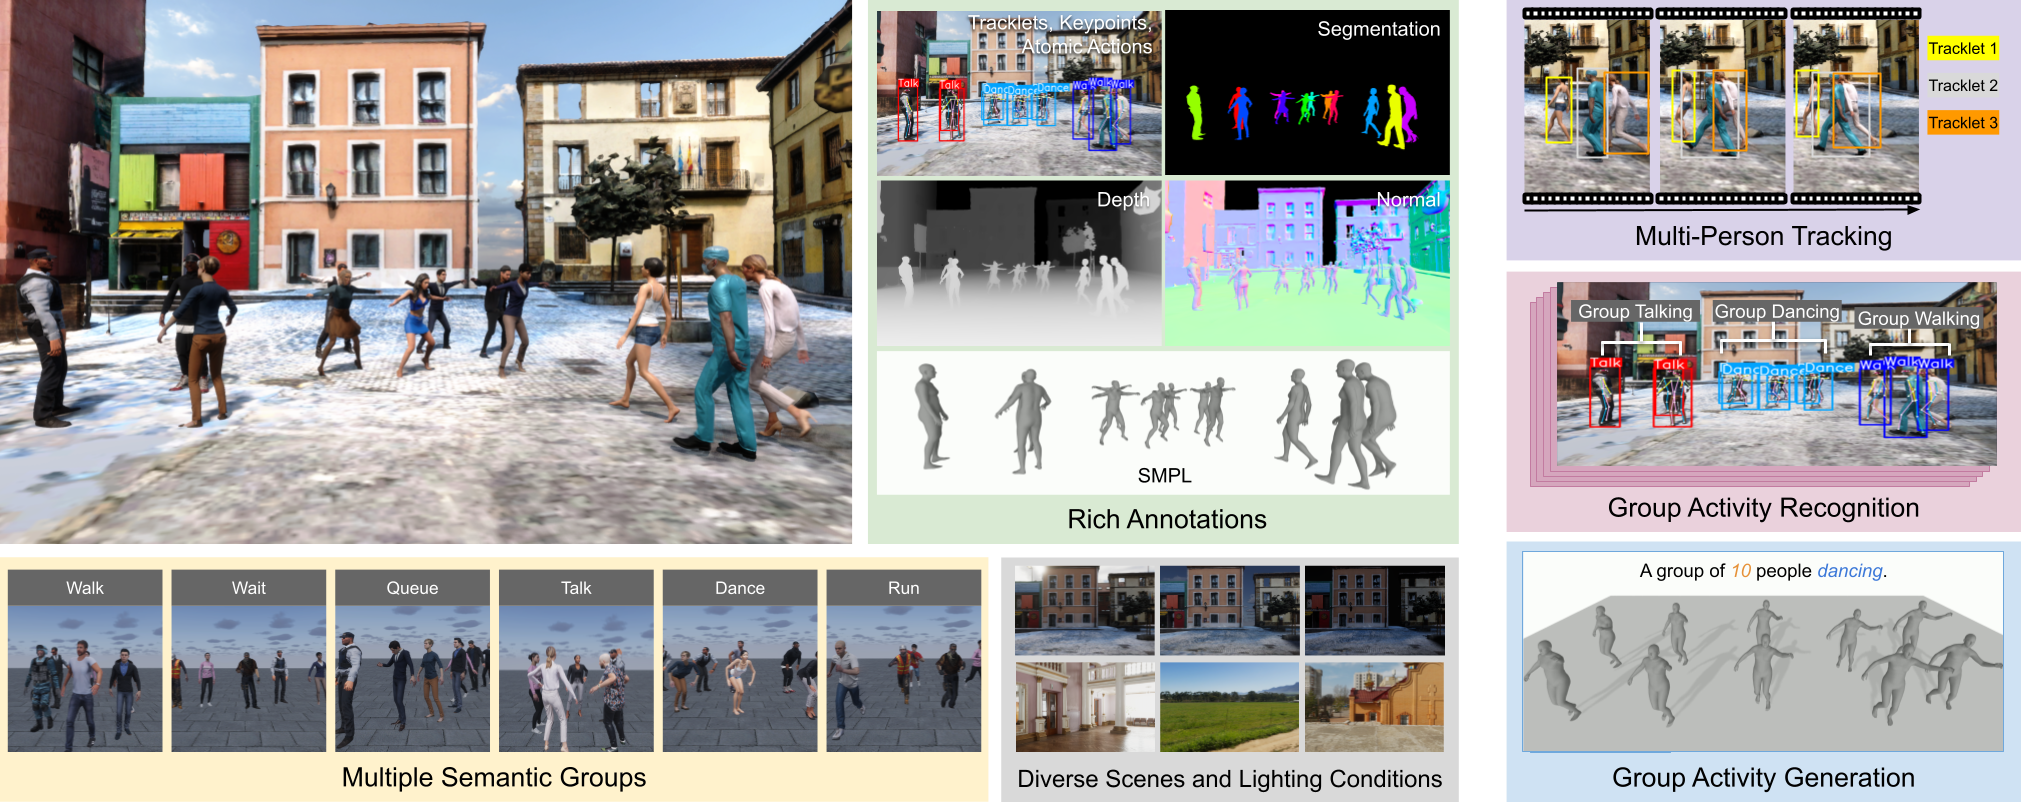
\includegraphics[width=0.85\linewidth]{pic/m3act.png}
    \caption[نمونه‌هایی از داده‌های مصنوعی تولید شده توسط چارچوب \lr{M3Act}]{نمونه‌هایی از داده‌های مصنوعی تولید شده توسط چارچوب \lr{M3Act}\protect\footnotemark}
    \label{fig:figm3act}
\end{figure}

\LTRfootnotetext{https://cjerry1243.github.io/M3Act/}

با وجود مزایای این رویکرد، پیاده‌سازی چنین سیستم‌هایی مستلزم استفاده از مدل‌های مولد پیچیده و منابع محاسباتی بسیار بالا \LTRfootnote{High Computational Cost} است که اجرای آن‌ها در مقیاس پروژه‌های کارشناسی عملاً امکان‌پذیر نیست. از این‌رو، در این پژوهش تمرکز بر استفاده از مجموعه‌داده‌های آماده و روش‌های استاندارد یادگیری قرار داده شده است.

شایان ذکر است که در این پژوهش، به‌دلیل محدودیت‌های زمانی و منابع، از یک مجموعه‌داده‌ی آماده استفاده شده است و فرآیند کامل ساخت مجموعه‌داده به‌صورت عملی پیاده‌سازی نشده است؛ با این حال، درک این مراحل برای تحلیل نتایج و توسعه‌های آتی ضروری است.

\clearpage
\section{مدل‌های مورد بررسی}
\subsection{نوع یک: مدل‌های ترکیبی کانولوشنی--توالی‌محور}
\label{sec:cnn_sequence_models}

در این بخش، یک دسته از روش‌های مبتنی بر ترکیب استخراج ویژگی‌های بصری و مدل‌سازی توالی مورد بررسی قرار می‌گیرد. در این رویکرد، به‌جای استفاده‌ی مستقیم از فریم‌های خام ویدیویی، ابتدا هر فریم به یک نمایش عددی فشرده در فضای ویژگی نگاشت می‌شود و سپس این نمایش‌ها در قالب یک ساختار دنباله‌ای مورد پردازش قرار می‌گیرند.

به‌طور مشخص، در این چارچوب هر ویدیو به‌صورت یک دنباله از بردارهای ویژگی در سطح فریم نمایش داده می‌شود که این بردارها توسط یک شبکه‌ی عصبی کانولوشنی از پیش آموزش‌دیده\LTRfootnote{Pretrained Convolutional Neural Network} استخراج شده‌اند. در ادامه، این توالی ویژگی‌ها به یک مدل توالی‌محور \LTRfootnote{Sequence Model} وارد می‌شود تا وابستگی‌های زمانی\LTRfootnote{Temporal Dependencies} میان فریم‌ها مدل‌سازی گردد.

لازم به ذکر است که در این سطح از مدل‌سازی، انتخاب معماری توالی‌محور می‌تواند متنوع باشد و شامل شبکه‌های عصبی بازگشتی، مدل‌های مبتنی بر ترنسفورمر \LTRfootnote{Transformer-based Models} یا سایر روش‌های پیشرفته باشد. با این حال، در این پژوهش به‌منظور ایجاد یک خط مبنا \LTRfootnote{Baseline}، تمرکز بر روی مدل‌های بازگشتی قرار گرفته است.

\subsubsection{مدل 1: رمزگذار کانولوشنی + شبکه عصبی بازگشتی}
در این مدل، توالی ویژگی‌های استخراج‌شده به یک شبکه‌ی عصبی بازگشتی\LTRfootnote{Recurrent Neural Network (RNN)} داده می‌شود. این معماری به‌عنوان ساده‌ترین مدل توالی‌محور، توانایی محدودی در مدل‌سازی وابستگی‌های بلندمدت دارد، اما به‌عنوان یک مبنای مقایسه مورد استفاده قرار می‌گیرد.

\subsubsection{مدل 2: رمزگذار کانولوشنی + شبکه \lr{LSTM}}
در این ساختار، از شبکه‌ی حافظه‌ی کوتاه-بلندمدت\LTRfootnote{Long Short-Term Memory (LSTM)} برای مدل‌سازی توالی استفاده می‌شود. این مدل با بهره‌گیری از سازوکار دروازه‌ها\LTRfootnote{Gates}، قادر به حفظ اطلاعات در بازه‌های زمانی طولانی‌تر بوده و معمولاً عملکرد بهتری نسبت به RNN ساده ارائه می‌دهد.

\subsubsection{مدل 3: رمزگذار کانولوشنی + شبکه \lr{LSTM} دوطرفه}
در این مدل، از نسخه‌ی دوطرفه‌ی LSTM\LTRfootnote{Bidirectional LSTM (BiLSTM)} استفاده می‌شود که توالی را به‌صورت هم‌زمان در دو جهت زمانی (رو به جلو و معکوس) پردازش می‌کند. این ویژگی امکان بهره‌گیری از اطلاعات زمینه‌ای کامل‌تر را فراهم می‌سازد، هرچند ممکن است در داده‌های محدود منجر به بیش‌برازش شود.

به‌طور کلی، خط لوله‌ی این دسته از مدل‌ها شامل سه مرحله‌ی اصلی زیر است:

\begin{enumerate}
    \item استخراج ویژگی در سطح فریم با استفاده از یک رمزگذار کانولوشنی ثابت\LTRfootnote{Frozen CNN Encoder}
    \item مدل‌سازی توالی با استفاده از یک مدل توالی‌محور (در این پژوهش: \lr{RNN}، \lr{LSTM} و \lr{BiLSTM})
    \item طبقه‌بندی کنش‌ها با استفاده از یک لایه‌ی پیش‌بینی کاملاً متصل\LTRfootnote{Fully Connected Prediction Head}
\end{enumerate}

در نهایت، سیستم یک دنباله از فریم‌ها را به‌عنوان ورودی دریافت کرده و یکی از سه کلاس کنش شامل \lr{Red Card}، \lr{Scoring} و \lr{Tackling} را به‌عنوان خروجی تولید می‌کند.

\subsection{نوع دو: مدل مبتنی بر ترنسفورمر فضایی-زمانی}

در این بخش، معماری \lr{TimeSformer} \cite{bertasius2021timesformer} به‌عنوان یکی از مدل‌های مبتنی بر ترنسفورمر برای مسئله تشخیص فعالیت گروهی در ویدیوهای ورزشی مورد بررسی قرار می‌گیرد. برخلاف مدل‌های مبتنی بر شبکه‌های کانولوشنی سه‌بعدی یا معماری‌های ترکیبی \lr{CNN+RNN} که وابستگی زمانی را به‌صورت ترتیبی مدل‌سازی می‌کنند، مدل \lr{TimeSformer} با تکیه بر سازوکار خودتوجه قادر است روابط فضایی و زمانی را به‌صورت همزمان و سراسری استخراج کند. این ویژگی باعث می‌شود که مدل بتواند وابستگی‌های بلندمدت میان فریم‌ها و همچنین تعاملات پیچیده میان بازیکنان را با دقت بیشتری مدل‌سازی نماید.

در مسئله تحلیل ویدیوهای ورزشی، رخدادهایی مانند گل، تکل یا کارت قرمز تنها وابسته به یک فریم خاص نیستند، بلکه توالی حرکات بازیکنان، موقعیت توپ، تغییرات صحنه و تعاملات جمعی در طول زمان نقش مهمی در تشخیص رویداد دارند. به همین دلیل، استفاده از معماری‌های مبتنی بر ترنسفورمر و توجه فضایی-زمانی می‌تواند عملکرد بهتری نسبت به مدل‌های سنتی ارائه دهد.

مدل مورد استفاده در این پژوهش، نسخه پایه \lr{TimeSformer} مبتنی بر معماری \lr{Vision Transformer (ViT)} \cite{dosovitskiy2021image} است که برای پردازش ویدیو توسعه داده شده است. این مدل، ویدیو را به‌عنوان دنباله‌ای از پچ‌\LTRfootnote{Patch}های تصویری در طول زمان در نظر گرفته و وابستگی‌های میان آن‌ها را از طریق لایه‌های توجه چندسری استخراج می‌کند.

\begin{figure}[H]
    \centering
    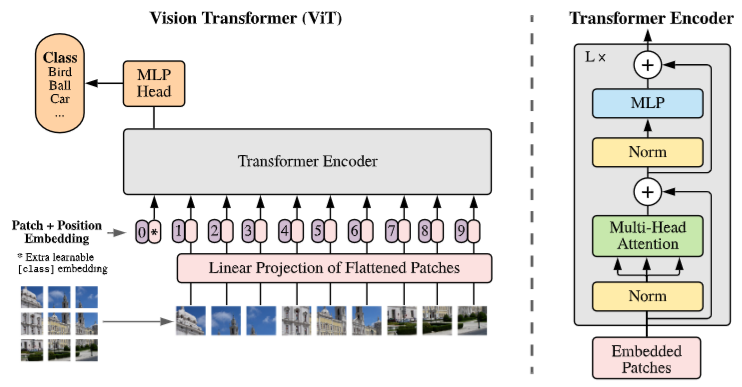
\includegraphics[width=0.75\linewidth]{pic/vit.png}
    \caption[معماری ویژن ترنسفورمر]{معماری ویژن ترنسفورمر\cite{dosovitskiy2021image}}
    \label{fig:placeholder}
\end{figure}

\subsubsection{مراحل آماده‌سازی داده‌ها}

در مرحله نخست، ویدیوهای مجموعه‌داده به تعداد مشخصی فریم نمونه‌برداری شدند. به‌منظور حفظ اطلاعات حرکتی و کاهش پیچیدگی محاسباتی، از هر ویدیو تعداد ثابتی فریم استخراج شد تا تمامی نمونه‌ها دارای طول یکسان باشند. سپس اندازه تمامی فریم‌ها به ابعاد ثابت تغییر داده شد تا ورودی استاندارد برای مدل فراهم گردد.

پس از استخراج فریم‌ها، عملیات نرمال‌سازی روی تصاویر اعمال شد. در این مرحله، مقادیر پیکسل‌ها بر اساس میانگین و انحراف معیار مجموعه‌داده \lr{ImageNet} تنظیم شدند تا مدل بتواند از وزن‌های اولیه از پیش آموزش‌دیده استفاده کند. علاوه بر این، به‌منظور جلوگیری از بیش‌برازش و افزایش تنوع داده‌ها، برخی تبدیلات داده مانند تغییر اندازه و برش استاندارد روی فریم‌ها اعمال شد.

هر ویدیو در نهایت به یک بردار چهار‌بعدی شامل تعداد فریم‌ها، کانال‌های رنگی، ارتفاع و عرض تصویر تبدیل شد. این بردار به‌عنوان ورودی به مدل \lr{TimeSformer} داده شد.

\subsubsection{معماری مدل}
معماری \lr{TimeSformer} مبتنی بر تقسیم هر فریم به مجموعه‌ای از پچ‌های کوچک تصویری است. هر پچ پس از تخت‌سازی\LTRfootnote{Flattening}، به یک بردار ویژگی تبدیل می‌شود. سپس تمامی بردارها به همراه کدگذاری مکانی و زمانی وارد بلوک‌های ترنسفورمر می‌شوند.

در هر بلوک ترنسفورمر، عملیات توجه خودکار فضایی و زمانی انجام می‌شود. توجه فضایی، ارتباط میان نواحی مختلف یک فریم را استخراج می‌کند و توجه زمانی، وابستگی میان فریم‌های مختلف را مدل‌سازی می‌نماید. این ساختار باعث می‌شود مدل بتواند الگوهای حرکتی و تعاملات گروهی را در طول زمان یاد بگیرد.

در انتهای معماری، خروجی توکن طبقه‌بندی به یک لایه کاملاً متصل داده می‌شود تا کلاس نهایی فعالیت پیش‌بینی گردد.

\subsubsection{راهبرد آموزش مدل}
به‌منظور بهره‌گیری از دانش اولیه مدل، از وزن‌های از پیش آموزش‌دیده روی مجموعه‌داده‌های بزرگ ویدیویی استفاده شد. سپس مدل روی مجموعه‌داده ورزشی این پژوهش بازآموزی\LTRfootnote{Fine-tuning} شد.

برای آموزش مدل از تابع هزینه \lr{Cross Entropy Loss} استفاده شد. همچنین بهینه‌سازی پارامترها با استفاده از الگوریتم \lr{AdamW} انجام گرفت که برای مدل‌های مبتنی بر ترنسفورمر عملکرد پایدارتری ارائه می‌دهد. نرخ یادگیری اولیه به‌صورت کوچک تنظیم شد تا فرآیند ریزتنظیم مدل با ثبات بیشتری انجام شود.

به‌دلیل پیچیدگی بالای معماری ترنسفورمر و محدود بودن حجم داده‌ها، استفاده از وزن‌های اولیه از پیش آموزش‌دیده نقش مهمی در همگرایی مدل داشت. علاوه بر این، اندازه دسته‌های آموزشی متناسب با محدودیت حافظه پردازنده گرافیکی انتخاب شد.

\subsubsection{فرآیند کلی اجرای مدل}

فرآیند کلی اجرای مدل \lr{TimeSformer} در این پژوهش مطابق شکل زیر انجام شده است:

\begin{figure}[H] 
\centering 
\begin{tikzpicture}[
    node distance=1.8cm, 
    every node/.style={font=\small}, 
    block/.style={rectangle, draw, rounded corners, minimum width=5cm, minimum height=1cm, align=center}, 
    arrow/.style={->, thick}
]

\node[block] (data) {\rl{ویدیوهای ورودی}}; 
\node[block, below of=data] (frames) {\rl{نمونه‌برداری فریم‌ها}}; 
\node[block, below of=frames] (pre) {\rl{تغییر اندازه و نرمال‌سازی}}; 
\node[block, below of=pre] (patch) {\rl{تبدیل فریم‌ها به پچ‌های تصویری}}; 
\node[block, below of=patch] (transformer) {\rl{استخراج ویژگی با \lr{TimeSformer}}}; 
\node[block, below of=transformer] (fc) {\rl{طبقه‌بندی کنش}}; 

\draw[arrow] (data) -- (frames); 
\draw[arrow] (frames) -- (pre); 
\draw[arrow] (pre) -- (patch); 
\draw[arrow] (patch) -- (transformer); 
\draw[arrow] (transformer) -- (fc); 

\end{tikzpicture} 
\caption{\rl{مراحل اصلی مدل مبتنی بر ترنسفورمر فضایی-زمانی}} 
\end{figure}

در این فرآیند، ابتدا فریم‌های کلیدی از هر ویدیو استخراج می‌شوند. سپس داده‌ها پس از پیش‌پردازش به پچ‌های تصویری تبدیل شده و وارد بلوک‌های ترنسفورمر می‌شوند. در ادامه، ویژگی‌های فضایی-زمانی استخراج شده و در نهایت کلاس فعالیت ورزشی توسط لایه طبقه‌بندی تعیین می‌شود.

\subsubsection{مزایا و محدودیت‌های مدل}

مهم‌ترین مزیت مدل \lr{TimeSformer} توانایی آن در مدل‌سازی وابستگی‌های بلندمدت زمانی و روابط پیچیده فضایی میان بازیکنان است. برخلاف معماری‌های مبتنی بر کانولوشن که معمولاً دارای میدان دید محدود هستند، سازوکار توجه در ترنسفورمر امکان بررسی کل توالی ویدیو را فراهم می‌کند.

همچنین این مدل قابلیت استفاده از وزن‌های از پیش آموزش‌دیده را دارد که در شرایط محدود بودن داده‌ها بسیار مؤثر است. از سوی دیگر، پیچیدگی محاسباتی بالا و نیاز به حافظه زیاد از جمله محدودیت‌های اصلی این معماری محسوب می‌شود. به همین دلیل، انتخاب تعداد فریم‌ها و اندازه ورودی تأثیر مستقیمی بر هزینه محاسباتی مدل دارد.


\section{صورت‌بندی مسئله}
\label{sec:problem_formulation}

یک ویدیو به‌صورت یک دنباله از $T$ فریم نمایش داده می‌شود:

\[
V = [I_1, I_2, \dots, I_T]
\]

در اینجا، هر فریم $I_t$ با استفاده از یک استخراج‌کننده‌ی ویژگی از پیش آموزش‌دیده \LTRfootnote{Pretrained Feature Extractor} به یک بردار ویژگی نگاشت می‌شود:

\[
x_t = f_{enc}(I_t), \quad x_t \in \mathbb{R}^{512}
\]

بنابراین، هر ویدیو به‌صورت یک دنباله از ویژگی‌ها نمایش داده می‌شود:

\[
X = [x_1, x_2, \dots, x_T], \quad X \in \mathbb{R}^{T \times 512}
\]

هدف این مسئله، یادگیری یک نگاشت \LTRfootnote{Mapping} از فضای توالی ویژگی‌ها به فضای برچسب‌ها است:

\[
f(X) \rightarrow y
\]

که در آن $y \in \{1,2,3\}$ متناظر با کلاس‌های زیر است:

\begin{itemize}
    \item کارت قرمز\LTRfootnote{Red Card} 
    \item گل زنی\LTRfootnote{Scoring}
    \item تکل زدن (یا تقابل فیزیکی برای تصاحب توپ)\LTRfootnote{Tackling}
    % \item و ...
\end{itemize}

این مسئله به‌صورت یک مسئله‌ی طبقه‌بندی چندکلاسه‌ی نظارت‌شده بر روی داده‌های توالی \LTRfootnote{Supervised Multi-class Sequence Classification} فرموله می‌شود.

\chapter{ارزیابی و تحلیل نتایج}

در این فصل، عملکرد مدل‌های پیشنهادی و آزمایش‌شده در این پژوهش مورد بررسی و ارزیابی قرار می‌گیرد. ابتدا با تحلیل آماری مجموعه‌داده‌ها، درک بهتری از توزیع داده‌ها و چالش‌های موجود حاصل می‌شود. سپس معیارهای ارزیابی مورد استفاده معرفی شده و اهمیت هر یک در سنجش عملکرد مدل‌ها تشریح می‌گردد. این معیارها مبنای مقایسه مدل‌ها در بخش‌های بعدی خواهند بود و به تفسیر دقیق‌تر نتایج کمک می‌کنند.

\section{تحلیل آماری مجموعه‌داده‌}

مجموعه‌داده‌ی مورد استفاده در این پژوهش از یک منبع عمومی در \lr{\href{https://www.kaggle.com/datasets/itarek898/football-match-actions-video-dataset}{Kaggle\LTRfootnote{https://www.kaggle.com/datasets/itarek898/football-match-actions-video-dataset}}} استخراج شده و شامل ویدیوهای کوتاه از مسابقات فوتبال با برچسب‌های کنشی می‌باشد. این مجموعه‌داده به سه بخش آموزش \LTRfootnote{Training}، اعتبارسنجی \LTRfootnote{Validation} و ارزیابی \LTRfootnote{Evaluation} تقسیم شده است.

\begin{figure}[H]
    \centering
    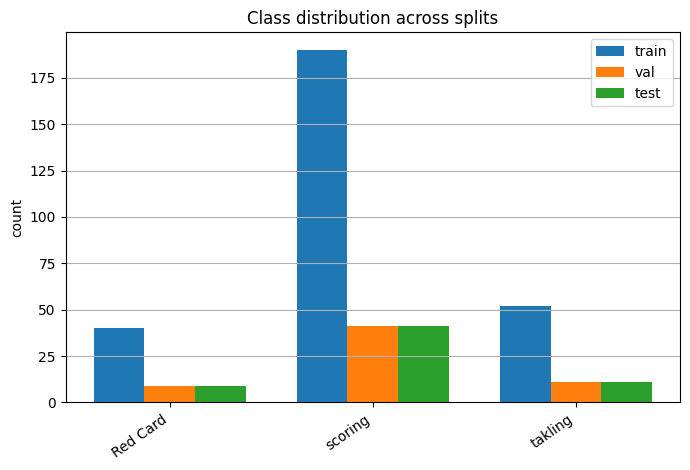
\includegraphics[width=0.75\linewidth]{pic/split_distribution.png}
    \caption[نمودار میله‌ای توزیع کلاس‌های دیتاست کنش‌های فوتبالی]{نمودار میله‌ای\footnotemark\space توزیع کلاس‌های دیتاست کنش‌های فوتبالی} 
    \label{fig:football_dist}
\end{figure}

\LTRfootnotetext{Bar Chart}

% همانطور که شکل \ref{fig:football_dist} نشان میدهد، بخش ارزیابی شامل ۶۱ نمونه بوده و توزیع کلاس‌ها در آن به‌صورت زیر است:

% \begin{itemize}
%     \item کارت قرمز: 9 نمونه
%     \item گل زنی: 41 نمونه
%     \item تکل زدن: 11 نمونه
% \end{itemize}

همان‌طور که شکل \ref{fig:football_dist} نشان می‌دهد، مجموعه‌داده دارای عدم توازن کلاس‌ها است؛ به‌طوری که کلاس گل‌زنی دارای بیشترین تعداد نمونه بوده و به‌طور قابل توجهی از سایر کلاس‌ها غالب‌تر است. اما نکته خوب ماجرا اینجاست که توزیع نمونه‌ها در همه بخش‌های داده (آموزش، ارزیابی و آزمایش) تا حدود زیادی مشابه است. این‌نکته گرچه ساده بنظر می‌رسد، اما نقش بسزایی در عملکرد مدل دارد. باید توجه داشت که در یکسری از اوقات این فرض صادق نیست و باید راهکارهای مقتضی را بکار گرفت تا نقش عدم توازن کلاس‌ها را کمرنگ کرد. از جمله این روشها میتوان به روش «زیرنمونه‌گیری منفی\LTRfootnote{Negative Subsampling}» اشاره کرد

در رویکرد زیرنمونه‌گیری منفی، از میان کلاس‌هایی با تعداد نمونه‌ی بسیار بالا، بخشی از داده‌ها به‌صورت تصادفی حذف می‌گردند تا توزیع نمونه‌ها در تمامی طبقه‌ها به تعادل نزدیک‌تر شود. این امر علاوه بر کاهش هزینه‌های محاسباتی، از غلبه‌ی کلاس‌های پرجمعیت بر فرایند آموزش جلوگیری کرده و منجر به بهبود توانایی مدل در تشخیص دقیق‌تر کلاس‌های اقلیت و استخراج ویژگی‌های تمایزگذار در تمامی دسته‌ها می‌شود.

\begin{figure}[H]
    \centering
    
    \begin{subfigure}[b]{0.65\textwidth}
        \centering
        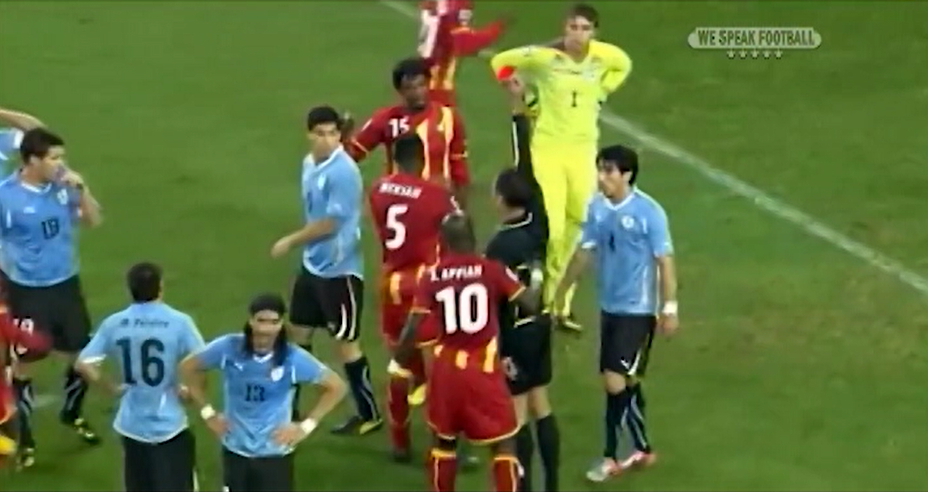
\includegraphics[width=\textwidth]{pic/redcard17.png}
        \caption{تصویر اول: فریمی از صحنه دریافت کارت قرمز}
    \end{subfigure}
    \hfill
    \begin{subfigure}[b]{0.65\textwidth}
        \centering
        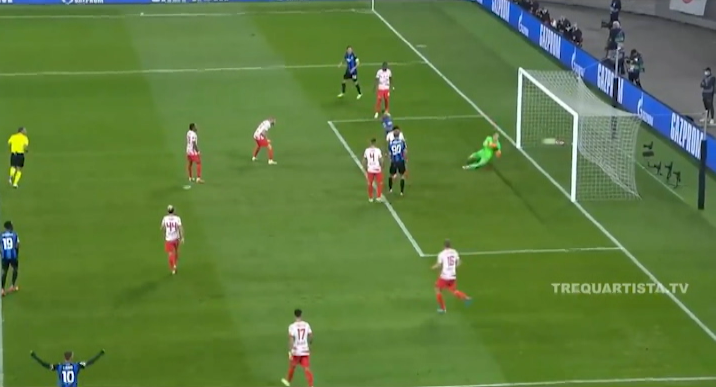
\includegraphics[width=\textwidth]{pic/scoring107.png}
        \caption{تصویر دوم: فریمی از صحنه به ثمر رسیدن گل}
    \end{subfigure}
    \hfill
    \begin{subfigure}[b]{0.65\textwidth}
        \centering
        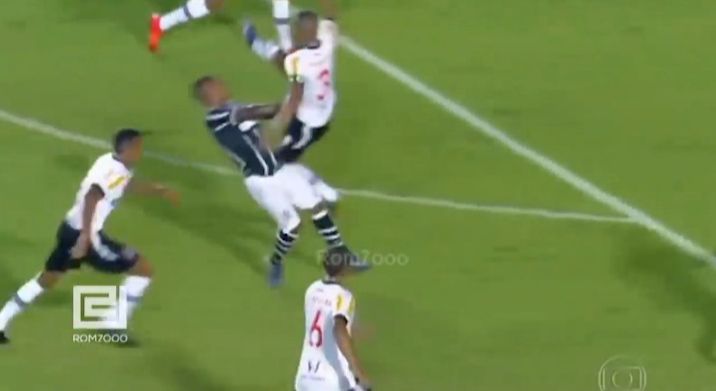
\includegraphics[width=\textwidth]{pic/tackle16.png}
        \caption{تصویر سوم: فریمی از صحنه‌ی یک درگیری فوتبالی}
    \end{subfigure}

    \caption{چند نمونه از دیتاست کنش‌های فوتبالی}
    \label{fig:three_images}
\end{figure}

در مجموع، تحلیل آماری مجموعه‌داده‌ها به درک بهتر ویژگی‌های داده، شناسایی چالش‌های بالقوه، و انتخاب مناسب‌تر روش‌های مدل‌سازی کمک می‌کند.

\section{معیارهای ارزیابی}

برای ارزیابی عملکرد مدل‌های طبقه‌بندی، استفاده از معیارهای مناسب ضروری است. در این پژوهش، از چهار معیار اصلی شامل دقت کلی، دقت به‌ازای هر کلاس، میانگین F1 ماکرو و میانگین F1 وزنی استفاده شده است. هر یک از این معیارها جنبه متفاوتی از عملکرد مدل را نشان می‌دهند و در کنار یکدیگر تصویر جامع‌تری ارائه می‌دهند.

\subsection[دقت کلی]{دقت کلی\LTRfootnote{Accuracy}}
دقت کلی یکی از ساده‌ترین و متداول‌ترین معیارهای ارزیابی در مسائل طبقه‌بندی است. این معیار نسبت تعداد پیش‌بینی‌های صحیح به کل نمونه‌ها را اندازه‌گیری می‌کند. دقت کلی دید کلی از عملکرد مدل ارائه می‌دهد و به‌ویژه زمانی که داده‌ها متوازن باشند، معیار مناسبی محسوب می‌شود.

با این حال، در شرایطی که توزیع کلاس‌ها نامتوازن باشد، دقت کلی می‌تواند گمراه‌کننده باشد. به‌عنوان مثال، اگر یک کلاس به‌طور قابل توجهی غالب باشد، مدلی که همواره آن کلاس را پیش‌بینی می‌کند ممکن است دقت بالایی داشته باشد، در حالی که عملکرد واقعی آن ضعیف است.

\subsection[دقت به‌ازای هر کلاس]{دقت به‌ازای هر کلاس\LTRfootnote{Per-Class Accuracy}}
برای رفع محدودیت‌های دقت کلی، بررسی دقت به‌ازای هر کلاس اهمیت پیدا می‌کند. این معیار عملکرد مدل را به‌صورت جداگانه برای هر کلاس ارزیابی می‌کند و نشان می‌دهد که مدل تا چه حد قادر به تشخیص صحیح نمونه‌های هر کلاس است.

این معیار به‌ویژه در مسائل نامتوازن اهمیت دارد، زیرا می‌تواند نشان دهد که آیا مدل نسبت به یک کلاس خاص سوگیری دارد یا خیر. تحلیل این معیار به شناسایی نقاط ضعف مدل کمک کرده و امکان بهبود هدفمند را فراهم می‌سازد.

\subsection[صحت]{صحت\LTRfootnote{Precision}}
معیار صحت که با نام ارزش پیش‌بینی مثبت\LTRfootnote{Positive Predictive Value} نیز شناخته می‌شود، به ارزیابی میزان دقت مدل در برچسب‌گذاری نمونه‌های مثبت می‌پردازد. به عبارت دیگر، این شاخص مشخص می‌کند که از میان تمامی نمونه‌هایی که توسط مدل به عنوان یک کنش خاص (مثلاً گل زدن) تشخیص داده شده‌اند، چه نسبتی واقعاً متعلق به آن طبقه بوده‌اند. بالا بودن میزان صحت به معنای کم بودن تعداد مثبت‌های کاذب\LTRfootnote{False Positives} است. این معیار طبق رابطه \ref{eq:precision} محاسبه می‌گردد:
\begin{equation}\label{eq:precision}
\text{Precision} = \frac{TP}{TP + FP}
\end{equation}
که در آن $TP$ تعداد مثبت‌های صحیح\LTRfootnote{True Positive} و $FP$ تعداد مثبت‌های کاذب است.

\subsection[بازخوانی]{بازخوانی\LTRfootnote{Recall}}
معیار بازخوانی یا حساسیت\LTRfootnote{Sensitivity}، بر توانایی مدل در بازیابی و شناسایی تمامی نمونه‌های مثبت موجود در مجموعه‌داده تمرکز دارد. در تشخیص کنش‌های فوتبالی، این معیار نشان می‌دهد که مدل تا چه حد موفق شده است تمامی رخدادهای واقعی (مثلاً تمام تکل‌های انجام شده در بازی) را شناسایی کند و چه میزان از آن‌ها را نادیده گرفته است. بالا بودن بازخوانی به معنای کم بودن تعداد منفی‌های کاذب\LTRfootnote{False Negatives} است. فرمول محاسباتی این معیار در رابطه \ref{eq:recall} آمده است:
\begin{equation}\label{eq:recall}
\text{Recall} = \frac{TP}{TP + FN}
\end{equation}
که در آن $FN$ نشان‌دهنده تعداد نمونه‌های مثبتی است که مدل به‌اشتباه آن‌ها را منفی تشخیص داده است.

\subsection[میانگین F1 ماکرو]{میانگین F1 ماکرو\LTRfootnote{Macro F1-Score}}
معیار F1 ترکیبی از دو معیار صحت\LTRfootnote{Precision} و بازخوانی\LTRfootnote{Recall} است و تعادلی میان این دو برقرار می‌کند. در حالت ماکرو، مقدار F1 برای هر کلاس به‌صورت جداگانه محاسبه شده و سپس میانگین آن‌ها گرفته می‌شود.

\begin{equation}
\text{\lr{Macro F1}} = \frac{1}{N} \sum_{i=1}^{N} F1_i
\end{equation}
که در آن $N$ تعداد کل کلاس‌ها است.

ویژگی مهم میانگین ماکرو این است که به همه کلاس‌ها وزن یکسانی می‌دهد، صرف‌نظر از تعداد نمونه‌های آن‌ها. بنابراین، این معیار برای ارزیابی عملکرد مدل در کلاس‌های کم‌نمونه بسیار مناسب است و دیدی منصفانه از عملکرد کلی ارائه می‌دهد.

\subsection[میانگین F1 وزنی]{میانگین F1 وزنی\LTRfootnote{Weighted F1-Score}}
در مقابل، میانگین F1 وزنی با در نظر گرفتن تعداد نمونه‌های هر کلاس محاسبه می‌شود. به این صورت که مقدار F1 هر کلاس متناسب با اندازه آن کلاس وزن‌دهی شده و سپس میانگین‌گیری انجام می‌شود.

\begin{equation}
\text{\lr{Weighted F1}} = \frac{\sum_{i=1}^{N} w_i \times F1_i}{\sum_{i=1}^{N} w_i}
\end{equation}
که در آن $w_i$ تعداد نمونه‌های متعلق به کلاس $i$-ام است.

این معیار بازتاب بهتری از عملکرد مدل در شرایط واقعی ارائه می‌دهد، زیرا تأثیر کلاس‌های پرنمونه را بیشتر در نظر می‌گیرد. در نتیجه، ترکیب این معیار با F1 ماکرو امکان تحلیل دقیق‌تری از رفتار مدل در مواجهه با داده‌های نامتوازن فراهم می‌سازد.


\clearpage
\section{مقایسه عملکرد مدل‌ها}

در این بخش، عملکرد مدل‌های مختلف مورد استفاده در این پژوهش به‌صورت کمی و کیفی مورد بررسی قرار می‌گیرد. برای هر مدل، نتایج حاصل از معیارهای ارزیابی شامل دقت کلی، میانگین F1 ماکرو و وزنی، و همچنین عملکرد به‌ازای هر کلاس گزارش می‌شود. علاوه بر این، با استفاده از جداول و تحلیل‌های تفصیلی، نقاط قوت و ضعف هر مدل در تشخیص کلاس‌های مختلف مورد بررسی قرار می‌گیرد. این تحلیل‌ها زمینه را برای مقایسه نهایی مدل‌ها و انتخاب بهترین رویکرد فراهم می‌کنند.

\subsection{مدل 1: رمزگذار کانولوشنی + شبکه عصبی بازگشتی}

در این مدل، از ترکیب شبکه‌های کانولوشنی برای استخراج ویژگی‌های مکانی و شبکه‌های عصبی بازگشتی برای مدل‌سازی وابستگی‌های زمانی استفاده شده است. این ساختار به‌ویژه برای تحلیل داده‌های ویدیویی مناسب است، زیرا قادر است هم اطلاعات فریم‌ها و هم توالی زمانی آن‌ها را در نظر بگیرد.

نتایج ارزیابی این مدل در جدول \ref{tab:cnn_rnn_results} ارائه شده است.

\begin{table}[h]
\centering
\caption{نتایج کلی مدل CNN+RNN}
\label{tab:cnn_rnn_results}
\begin{tabular}{c|c|c}
\hline
دقت & F1 ماکرو & F1 وزنی \\
\hline
\lr{0.8525} & \lr{0.7670} & \lr{0.8426} \\   
\hline
\end{tabular}
\end{table}

برای تحلیل دقیق‌تر، عملکرد مدل به تفکیک هر کلاس در جدول \ref{tab:cnn_rnn_class} نشان داده شده است.

\begin{table}[h]
\centering
\caption{عملکرد مدل CNN+RNN به‌ازای هر کلاس}
\label{tab:cnn_rnn_class}
\begin{tabular}{c|c|c|c|c|c}
\hline
کلاس & دقت & صحت & بازخوانی & F1 ماکرو & تعداد نمونه \\
\hline
کارت قرمز & \lr{0.6667} & \lr{0.8571} & \lr{0.6667} & \lr{0.7500} & \lr{9} \\ \hline
گل & \lr{0.9756} & \lr{0.8696} & \lr{0.9756} & \lr{0.9195} & \lr{41} \\ \hline
تکل & \lr{0.5455} & \lr{0.7500} & \lr{0.5455} & \lr{0.6316} & \lr{11} \\ \hline
\end{tabular}
\end{table}

\begin{figure}[H]
    \centering
    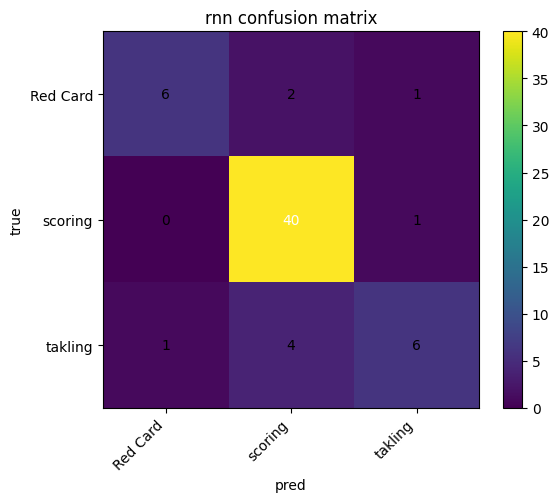
\includegraphics[width=0.75\linewidth]{pic/rnn_cm.png}
    \caption[ماتریس درهم‌ریختگی عملکرد مدل CNN+RNN روی داده‌های آزمایش]{ماتریس درهم‌ریختگی\footnotemark عملکرد مدل CNN+RNN روی داده‌های آزمایش\protect}
    \label{fig:rnn_cm}
\end{figure}
\LTRfootnotetext{\lr{Confusion Matrix}}

با توجه به نتایج به‌دست‌آمده، این مدل عملکرد مناسبی در تشخیص کلاس «گل» از خود نشان می‌دهد. مقدار بالای بازخوانی و F1 ماکرو برای این کلاس نشان می‌دهد که مدل قادر است اغلب نمونه‌های مربوط به گل را به‌درستی شناسایی کند. این موضوع احتمالاً به دلیل فراوانی بیشتر نمونه‌های این کلاس در مجموعه‌داده و الگوهای مشخص‌تر آن در داده‌های ویدیویی است.

در مقابل، عملکرد مدل در کلاس‌های «کارت قرمز» و «تکل» ضعیف‌تر است. به‌ویژه در کلاس «تکل»، مقدار بازخوانی پایین (0.5455) نشان می‌دهد که تعداد قابل توجهی از نمونه‌های این کلاس به‌درستی شناسایی نشده‌اند. این مسئله می‌تواند ناشی از شباهت بصری این رویداد با سایر کنش‌ها یا تعداد کمتر نمونه‌های آموزشی باشد.

همچنین اختلاف قابل توجه بین F1 ماکرو (\lr{0.7670}) و F1 وزنی (\lr{0.8426}) نشان‌دهنده تأثیر عدم توازن داده‌ها است. از آنجا که کلاس «گل» سهم بیشتری از داده‌ها را دارد و عملکرد مدل در این کلاس بسیار خوب است، مقدار F1 وزنی افزایش یافته است، در حالی که F1 ماکرو تصویر واقع‌بینانه‌تری از عملکرد مدل در تمامی کلاس‌ها ارائه می‌دهد.

به‌طور کلی، این مدل در یادگیری الگوهای غالب موفق عمل کرده، اما در تشخیص کلاس‌های کم‌نمونه و پیچیده‌تر با چالش مواجه است.



\subsection{مدل 2: رمزگذار کانولوشنی + LSTM}

در این مدل، به‌جای استفاده از شبکه بازگشتی ساده، از معماری LSTM به‌منظور مدل‌سازی وابستگی‌های زمانی بلندمدت استفاده شده است. LSTM به دلیل داشتن ساختار حافظه‌دار، قادر است اطلاعات مهم را در طول توالی حفظ کرده و وابستگی‌های پیچیده‌تری را نسبت به شبکه‌های عصبی بازگشتی ساده یاد بگیرد. این ویژگی به‌ویژه در تحلیل ویدیوهای ورزشی که شامل توالی‌های زمانی معنادار هستند، اهمیت دارد.

نتایج کلی این مدل در جدول \ref{tab:cnn_lstm_results} ارائه شده است.

\begin{table}[h]
\centering
\caption{نتایج کلی مدل CNN+LSTM}
\label{tab:cnn_lstm_results}
\begin{tabular}{c|c|c}
\hline
دقت & F1 ماکرو & F1 وزنی \\
\hline
\lr{0.9344} & \lr{0.8989} & \lr{0.9321} \\
\hline
\end{tabular}
\end{table}

عملکرد مدل به تفکیک هر کلاس در جدول \ref{tab:cnn_lstm_class} نشان داده شده است.

\begin{table}[h]
\centering
\caption{عملکرد مدل CNN+LSTM به‌ازای هر کلاس}
\label{tab:cnn_lstm_class}
\begin{tabular}{c|c|c|c|c|c}
\hline
کلاس & دقت & صحت & بازخوانی & F1 ماکرو & تعداد نمونه \\
\hline
کارت قرمز & \lr{0.7778} & \lr{1.0000} & \lr{0.7778} & \lr{0.8750} & \lr{9} \\
گل & \lr{1.0000} & \lr{0.9318} & \lr{1.0000} & \lr{0.9647} & \lr{41} \\
تکل & \lr{0.8182} & \lr{0.9000} & \lr{0.8182} & \lr{0.8571} & \lr{11} \\
\hline
\end{tabular}
\end{table}

\begin{figure}[H]
    \centering
    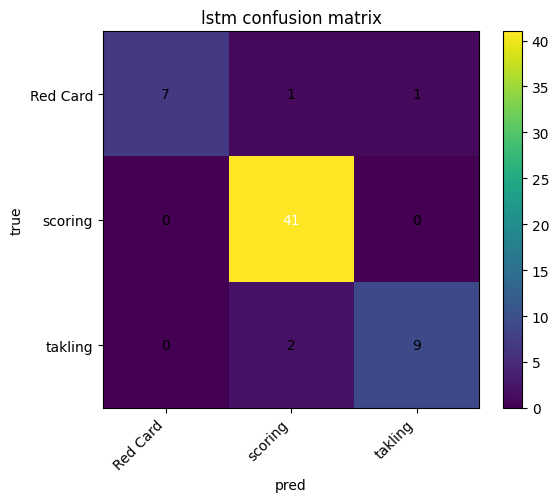
\includegraphics[width=0.75\linewidth]{pic/lstm_cm.png}
    \caption{ماتریس درهم‌ریختگی عملکرد مدل CNN+LSTM روی داده‌های آزمایش}
    \label{fig:placeholder}
\end{figure}

با توجه به نتایج به‌دست‌آمده، این مدل نسبت به مدل قبلی بهبود قابل توجهی در تمامی معیارها نشان می‌دهد. دقت کلی از مقدار \lr{0.8525} به \lr{0.9344} افزایش یافته و مقدار F1 ماکرو نیز به \lr{0.8989} رسیده است که نشان‌دهنده بهبود عملکرد در تمامی کلاس‌ها، به‌ویژه کلاس‌های کم‌نمونه، است.

در کلاس «گل»، مدل عملکرد بسیار مطلوبی داشته و مقدار بازخوانی برابر با \lr{1.0000} نشان می‌دهد که تمامی نمونه‌های این کلاس به‌درستی شناسایی شده‌اند. همچنین مقدار F1-score بالا (\lr{0.9647}) بیانگر تعادل مناسب بین دقت و بازخوانی در این کلاس است.

در کلاس «کارت قرمز»، اگرچه مقدار صحت برابر با \lr{1.0000} است، اما بازخوانی برابر با \lr{0.7778} نشان می‌دهد که هنوز برخی نمونه‌ها شناسایی نشده‌اند. با این حال، نسبت به مدل قبلی، بهبود قابل توجهی مشاهده می‌شود.

بیشترین پیشرفت مربوط به کلاس «تکل» است، جایی که بازخوانی از \lr{0.5455} در مدل قبلی به \lr{0.8182} افزایش یافته است. این نشان می‌دهد که استفاده از LSTM توانسته وابستگی‌های زمانی پیچیده‌تر را بهتر مدل‌سازی کرده و در نتیجه عملکرد مدل در تشخیص این کلاس بهبود یابد.

همچنین نزدیکی مقادیر F1 ماکرو (\lr{0.8989}) و F1 وزنی (\lr{0.9321}) نشان می‌دهد که مدل عملکرد متعادلی در کلاس‌های مختلف دارد و تأثیر عدم توازن داده‌ها کاهش یافته است.

به‌طور کلی، جایگزینی RNN با LSTM منجر به بهبود چشمگیر در عملکرد مدل شده و نشان می‌دهد که استفاده از معماری‌های پیشرفته‌تر برای مدل‌سازی توالی زمانی در مسئله تشخیص فعالیت‌های گروهی بسیار مؤثر است.


\subsection{مدل 3: رمزگذار کانولوشنی + Bi-LSTM}

در این مدل، به‌منظور بهره‌گیری هم‌زمان از اطلاعات گذشته و آینده در توالی‌های زمانی، از معماری Bi-LSTM استفاده شده است. برخلاف LSTM یک‌جهته، این مدل توالی را در هر دو جهت زمانی پردازش می‌کند و در نتیجه انتظار می‌رود بتواند وابستگی‌های پیچیده‌تری را در داده‌های ویدیویی استخراج کند.

نتایج کلی این مدل در جدول \ref{tab:cnn_bilstm_results} ارائه شده است.

\begin{table}[h]
\centering
\caption{نتایج کلی مدل CNN+Bi-LSTM}
\label{tab:cnn_bilstm_results}
\begin{tabular}{c|c|c}
\hline
دقت & F1 ماکرو & F1 وزنی \\
\hline
\lr{0.8361} & \lr{0.7523} & \lr{0.8260} \\
\hline
\end{tabular}
\end{table}

عملکرد مدل به تفکیک هر کلاس در جدول \ref{tab:cnn_bilstm_class} نشان داده شده است.

\begin{table}[h]
\centering
\caption{عملکرد مدل CNN+Bi-LSTM به‌ازای هر کلاس}
\label{tab:cnn_bilstm_class}
\begin{tabular}{c|c|c|c|c|c}
\hline
کلاس & دقت & صحت & بازخوانی & F1 ماکرو & تعداد نمونه \\
\hline
کارت قرمز & \lr{0.7778} & \lr{0.8750} & \lr{0.7778} & \lr{0.8235} & \lr{9} \\
گل & \lr{0.9512} & \lr{0.8667} & \lr{0.9512} & \lr{0.9070} & \lr{41} \\
تکل & \lr{0.4545} & \lr{0.6250} & \lr{0.4545} & \lr{0.5263} & \lr{11} \\
\hline
\end{tabular}
\end{table}

\begin{figure}[H]
    \centering
    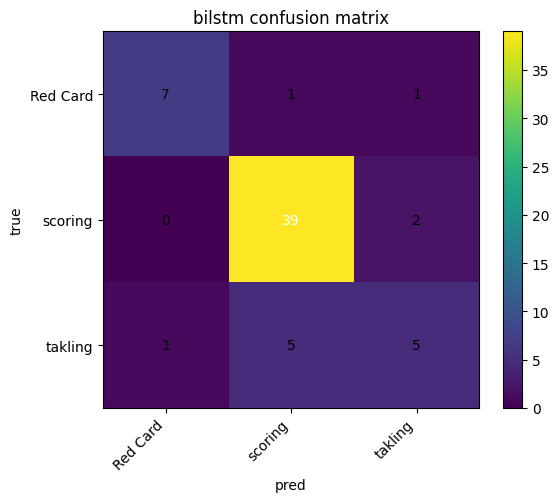
\includegraphics[width=0.75\linewidth]{pic/bilstm_cm.png}
    \caption{ماتریس درهم‌ریختگی عملکرد مدل CNN+Bi-LSTM روی داده‌های آزمایش}
    \label{fig:cm-}
\end{figure}

با توجه به نتایج، این مدل عملکرد ضعیف‌تری نسبت به مدل LSTM یک‌جهته از خود نشان داده است. دقت کلی برابر با \lr{0.8361} بوده که نسبت به مقدار \lr{0.9344} در مدل قبلی کاهش قابل توجهی دارد. همچنین مقدار F1 ماکرو (\lr{0.7523}) نشان‌دهنده افت عملکرد مدل در کلاس‌های مختلف، به‌ویژه کلاس‌های کم‌نمونه، است.

در کلاس «گل»، همچنان عملکرد مدل مناسب است و مقدار Recall برابر با \lr{0.9512} نشان می‌دهد که بخش عمده‌ای از نمونه‌های این کلاس به‌درستی شناسایی شده‌اند. با این حال، مقدار F1-score (\lr{0.9070}) نسبت به مدل LSTM کاهش یافته است.

در کلاس «کارت قرمز»، عملکرد مدل نسبتاً قابل قبول است و مقدار F1 برابر با \lr{0.8235} نشان می‌دهد که مدل توانسته تا حدی این کلاس را تشخیص دهد. 

بیشترین افت عملکرد مربوط به کلاس «تکل» است، جایی که مقدار بازخوانی به \lr{0.4545} کاهش یافته است. این موضوع نشان می‌دهد که مدل در تشخیص این کلاس با چالش جدی مواجه است و تعداد زیادی از نمونه‌های این کلاس را از دست داده است.

کاهش عملکرد این مدل را می‌توان به پیچیدگی بیشتر معماری Bi-LSTM و احتمال بیش‌برازش\LTRfootnote{Overfit} نسبت داد. همچنین، در مجموعه‌داده‌های با حجم محدود، استفاده از مدل‌های پیچیده‌تر لزوماً به بهبود عملکرد منجر نمی‌شود و حتی ممکن است باعث افت دقت شود.

به‌طور کلی، اگرچه Bi-LSTM از نظر تئوری قادر به استخراج اطلاعات بیشتری از توالی است، اما در این مسئله خاص و با توجه به ویژگی‌های مجموعه‌داده، عملکرد آن نسبت به LSTM یک‌جهته ضعیف‌تر بوده است.

\subsection{مدل 4: مدل مبتنی بر ترنسفورمر فضایی-زمانی}

در این بخش، عملکرد مدل مبتنی بر ترنسفورمر فضایی-زمانی \lr{TimeSformer} مورد بررسی قرار می‌گیرد. این معماری با استفاده از سازوکار توجه قادر است وابستگی‌های فضایی و زمانی را به‌صورت همزمان مدل‌سازی کند و در نتیجه برای تحلیل ویدیوهای ورزشی و تشخیص فعالیت‌های گروهی گزینه‌ای مناسب محسوب می‌شود.

برخلاف مدل‌های مبتنی بر شبکه‌های بازگشتی که اطلاعات زمانی را به‌صورت ترتیبی پردازش می‌کنند، در این معماری تمامی فریم‌ها به‌صورت همزمان مورد توجه قرار می‌گیرند. این ویژگی باعث می‌شود مدل بتواند تعاملات پیچیده میان بازیکنان و تغییرات صحنه را با دقت بیشتری استخراج کند.

نتایج کلی این مدل در جدول \ref{tab:timesformer_results} ارائه شده است.

\begin{table}[h]
\centering
\caption{نتایج کلی مدل \lr{TimeSformer}}
\label{tab:timesformer_results}
\begin{tabular}{c|c|c}
\hline
دقت & F1 ماکرو & F1 وزنی \\
\hline
\lr{1.0000} & \lr{1.0000} & \lr{1.0000} \\
\hline
\end{tabular}
\end{table}

عملکرد مدل به تفکیک هر کلاس در جدول \ref{tab:timesformer_class} نشان داده شده است.

\begin{table}[h]
\centering
\caption{عملکرد مدل \lr{TimeSformer} به‌ازای هر کلاس}
\label{tab:timesformer_class}
\begin{tabular}{c|c|c|c|c|c}
\hline
کلاس & دقت & صحت & بازخوانی & F1 ماکرو & تعداد نمونه \\
\hline
کارت قرمز & \lr{1.0000} & \lr{1.0000} & \lr{1.0000} & \lr{1.0000} & \lr{9} \\
گل & \lr{1.0000} & \lr{1.0000} & \lr{1.0000} & \lr{1.0000} & \lr{41} \\
تکل & \lr{1.0000} & \lr{1.0000} & \lr{1.0000} & \lr{1.0000} & \lr{11} \\
\hline
\end{tabular}
\end{table}

همان‌طور که مشاهده می‌شود، مدل \lr{TimeSformer} در تمامی معیارهای ارزیابی به عملکرد کامل دست یافته است. دقت کلی، F1 ماکرو و F1 وزنی همگی برابر با \lr{1.0000} هستند که نشان‌دهنده توانایی بسیار بالای مدل در تشخیص فعالیت‌های گروهی مختلف است.

در کلاس «گل»، مدل تمامی نمونه‌ها را به‌درستی شناسایی کرده و هیچ خطایی مشاهده نشده است. این موضوع نشان می‌دهد که معماری ترنسفورمر فضایی-زمانی توانسته الگوهای حرکتی و تغییرات صحنه مرتبط با این رخداد را به‌صورت کامل یاد بگیرد.

همچنین در کلاس‌های «کارت قرمز» و «تکل» نیز عملکرد مدل کاملاً بدون خطا بوده است. این نتیجه اهمیت استفاده از سازوکار توجه فضایی-زمانی را نشان می‌دهد، زیرا این معماری قادر است ارتباط میان بازیکنان، تغییرات موقعیتی و وابستگی‌های زمانی طولانی‌مدت را بهتر از انواع شبکه‌های عسبی بازگشتی استخراج کند.

\begin{figure}
    \centering
    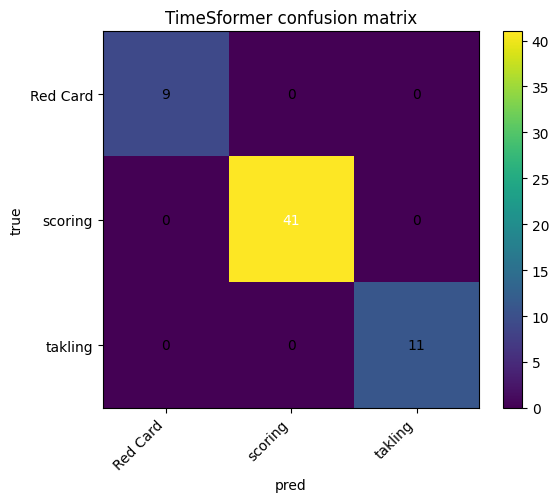
\includegraphics[width=0.75\linewidth]{pic/timesformer_cm.png}
    \caption{ماتریس درهم‌ریختگی عملکرد مدل TimeSformer روی داده‌های آزمایش}
    \label{fig:cm-TimeSformer}
\end{figure}

یکی از عوامل مهم در موفقیت این مدل، استفاده از وزن‌های از پیش آموزش‌دیده است. با توجه به محدود بودن اندازه مجموعه‌داده، آموزش کامل یک مدل ترنسفورمر از ابتدا می‌توانست منجر به بیش‌برازش شود؛ اما استفاده از دانش منتقل‌شده از مرحله پیش‌آموزش باعث افزایش پایداری آموزش و بهبود عملکرد نهایی شده است.

در مقایسه با مدل‌های قبلی، این معماری توانسته عملکرد بسیار بهتری ارائه دهد. در حالی که مدل‌های قبلی در برخی کلاس‌ها به‌ویژه «تکل» و «کارت قرمز» با افت عملکرد مواجه بودند، مدل \lr{TimeSformer} تمامی کلاس‌ها را با دقت کامل تشخیص داده است.

همچنین برخلاف معماری‌های بازگشتی که اطلاعات زمانی را به‌صورت ترتیبی منتقل می‌کنند و ممکن است بخشی از اطلاعات در توالی‌های طولانی از بین برود، سازوکار توجه در ترنسفورمر امکان تحلیل همزمان تمامی فریم‌ها را فراهم می‌کند. این ویژگی در تحلیل فعالیت‌های گروهی که وابستگی زمانی و تعامل میان بازیکنان اهمیت بالایی دارد، نقش مهمی ایفا می‌کند.

با وجود عملکرد بسیار بالا، باید توجه داشت که دستیابی به دقت کامل ممکن است تا حدی تحت تأثیر محدود بودن اندازه مجموعه‌داده و تعداد کم نمونه‌های آزمون نیز باشد. بنابراین، برای ارزیابی دقیق‌تر قابلیت تعمیم مدل، استفاده از مجموعه‌داده‌های بزرگ‌تر و متنوع‌تر در پژوهش‌های آینده ضروری خواهد بود.

به‌طور کلی، مدل \lr{TimeSformer} بهترین عملکرد را در میان تمامی مدل‌های بررسی‌شده ارائه داد و نشان داد که معماری‌های مبتنی بر ترنسفورمر فضایی-زمانی می‌توانند گزینه‌ای بسیار مؤثر برای مسئله تشخیص فعالیت گروهی در ویدیوهای ورزشی باشند.




\chapter{نتیجه‌گیری و چشم‌انداز آینده}

\section{نتیجه‌گیری}

در فصل‌های قبل به تفصیل توضیح داده شد که تشخیص فعالیت گروهی یکی از مسائل مهم و چالش‌برانگیز در حوزه بینایی ماشین و تحلیل ویدیو به شمار می‌رود که هدف آن، درک رفتار جمعی افراد و تحلیل تعاملات میان آن‌ها در یک صحنه پویا است. این مسئله در کاربردهای مختلفی مانند نظارت هوشمند، تحلیل رفتار اجتماعی، سامانه‌های امنیتی و به‌ویژه تحلیل مسابقات ورزشی اهمیت فراوانی دارد. در سناریوهای ورزشی، تشخیص صحیح فعالیت‌های گروهی می‌تواند در تحلیل تاکتیکی تیم‌ها، بررسی عملکرد بازیکنان، تولید خلاصه مسابقات و حتی کمک به تصمیم‌گیری مربیان مورد استفاده قرار گیرد.

با وجود پیشرفت‌های قابل‌توجه در سال‌های اخیر، مسئله تشخیص فعالیت گروهی همچنان با چالش‌های متعددی همراه است. از جمله این چالش‌ها می‌توان به پیچیدگی تعاملات میان افراد، تغییرات سریع حرکتی، انسداد بازیکنان، تنوع زاویه‌های دوربین، تغییرات نور، شباهت میان برخی فعالیت‌ها و محدود بودن مجموعه‌داده‌های تخصصی ورزشی اشاره کرد. علاوه بر این، بسیاری از فعالیت‌های گروهی وابستگی زمانی و فضایی پیچیده‌ای دارند که مدل‌سازی آن‌ها نیازمند استفاده از معماری‌های پیشرفته یادگیری عمیق است.

در این پژوهش، مسئله تشخیص فعالیت گروهی در ویدیوهای ورزشی مورد بررسی قرار گرفت و تلاش شد تا عملکرد چندین معماری یادگیری عمیق در این حوزه ارزیابی شود. در ابتدا، مجموعه‌داده‌ای از ویدیوهای مسابقات فوتبال تهیه و سازمان‌دهی شد که شامل چند کلاس مختلف از فعالیت‌های گروهی بود. فرآیند آماده‌سازی داده‌ها برای ساخت یک مجموعه‌داده مناسب برای انجام این‌چنین پروژه‌هایی توضیح داده شد که با چالش‌ها و سختی‌های زیادی شامل استخراج ویدیوها، یکسان‌سازی ساختار داده‌ها، دسته‌بندی نمونه‌ها و آماده‌سازی آن‌ها برای آموزش مدل‌ها همراه بود. با توجه به محدود بودن توان محاسباتی و اندازه مجموعه‌داده، طراحی آزمایش‌ها به‌گونه‌ای انجام شد که بتوان حداکثر بهره را از داده‌های موجود استخراج کرد.

پس از آماده‌سازی داده‌ها، چندین مدل مبتنی بر یادگیری عمیق مورد آزمایش قرار گرفتند. در ابتدا، مدل‌های مبتنی بر ترکیب شبکه‌های عصبی کانولوشنی و شبکه‌های عصبی بازگشتی بررسی شدند. این مدل‌ها توانایی مناسبی در استخراج ویژگی‌های حرکتی و الگوهای زمانی موجود در توالی فریم‌ها داشتند، اما در مدل‌سازی وابستگی‌های بلندمدت میان فریم‌ها محدودیت‌هایی مشاهده شد.

در ادامه، مدل TimeSformer به‌عنوان یک معماری مبتنی بر ترنسفورمر فضایی-زمانی مورد استفاده قرار گرفت. این مدل با استفاده از مکانیزم توجه قادر است روابط زمانی و فضایی میان فریم‌های ویدیویی را به‌صورت مؤثرتری مدل‌سازی کند. نتایج آزمایش‌ها نشان داد که مدل‌ \lr{TimeSformer}، عملکرد بسیارخوبی در مسئله تشخیص فعالیت گروهی ارائه می‌دهد و در استخراج وابستگی‌های پیچیده میان فریم‌ها موفق‌تر عمل می‌کنند.

ارزیابی نتایج نشان داد که کیفیت و تنوع داده‌ها تأثیر مستقیمی بر عملکرد مدل‌ها دارد. همچنین برخی کلاس‌های فعالیت به دلیل شباهت زیاد در الگوهای حرکتی یا محدود بودن نمونه‌های آموزشی، همچنان با نرخ خطای بالاتری همراه بودند. علاوه بر این، محدودیت منابع محاسباتی و حجم بالای پردازش ویدیو از دیگر چالش‌های مهم در اجرای مدل‌های پیشرفته محسوب می‌شد.

به‌طور کلی، نتایج این پژوهش نشان داد که استفاده از مدل‌های یادگیری عمیق، به‌ویژه معماری‌های مبتنی بر ترنسفورمر، می‌تواند رویکردی مؤثر برای تحلیل فعالیت‌های گروهی در ویدیوهای ورزشی باشد. همچنین این پژوهش بستری مناسب برای توسعه سامانه‌های هوشمند تحلیل مسابقات ورزشی و تحقیقات پیشرفته‌تر در حوزه تحلیل رفتار گروهی فراهم می‌کند.

\begin{table}[H]
\centering
\caption{تحلیل ساختاری و مقایسه‌ای معماری‌های تشخیص فعالیت گروهی}
\label{tab:model_comparison}

\scriptsize
\setlength{\tabcolsep}{3pt}
\renewcommand{\arraystretch}{1.4}

\begin{tabular}{|m{2.2cm}|m{1.5cm}|m{1.5cm}|m{1.5cm}|m{1.5cm}|m{2cm}|m{2cm}|}
\hline

\centering \textbf{معماری} &
\centering \textbf{استخراج ویژگی فضایی} &
\centering \textbf{مدل‌سازی زمانی} &
\centering \textbf{پیچیدگی محاسباتی} &
\centering \textbf{مناسب برای داده محدود} &
\centering \textbf{مزایا} &
\centering \textbf{محدودیت‌ها}
\tabularnewline
\hline

% \centering شبکه‌های کانولوشنی دوبعدی &
% \centering بالا &
% \centering ضعیف &
% \centering پایین تا متوسط &
% \centering مناسب &
% \centering سادگی و سرعت آموزش مناسب &
% \centering عدم توانایی درک مستقیم وابستگی زمانی
% \tabularnewline
% \hline

\centering شبکه‌های کانولوشنی سه‌بعدی &
\centering بالا &
\centering مناسب برای وابستگی کوتاه‌مدت &
\centering بالا &
\centering نسبتاً ضعیف &
\centering استخراج هم‌زمان اطلاعات حرکتی و فضایی &
\centering مصرف حافظه و محاسبات زیاد
\tabularnewline
\hline

\centering مدل‌های ترکیبی کانولوشنی-بازگشتی &
\centering بالا &
\centering مناسب &
\centering متوسط تا بالا &
\centering متوسط &
\centering تحلیل مناسب دنباله‌های زمانی &
\centering آموزش پیچیده و وابستگی به طول توالی
\tabularnewline
\hline

\centering ترنسفورمر فضایی-زمانی مثل TimeSformer &
\centering بسیار بالا &
\centering بسیار قوی &
\centering بسیار بالا &
\centering متوسط تا ضعیف &
\centering استفاده مؤثر از مکانیزم توجه &
\centering زمان آموزش بالا و نیازمند GPU قدرتمند
\tabularnewline
\hline

\centering شبکه‌های عصبی گرافی &
\centering مبتنی بر روابط میان افراد &
\centering قوی در تحلیل تعاملات &
\centering متوسط تا بالا &
\centering متوسط &
\centering مدل‌سازی تعاملات اجتماعی و گروهی &
\centering وابستگی به داده‌های ساختاریافته
\tabularnewline
\hline

\centering مدل‌های چندوجهی &
\centering بسیار بالا &
\centering قوی &
\centering بسیار بالا &
\centering ضعیف تا متوسط &
\centering استفاده هم‌زمان از اطلاعات مکمل &
\centering پیچیدگی طراحی و هماهنگ‌سازی داده‌ها
\tabularnewline
\hline

\end{tabular}
\end{table}

همان‌طور که در جدول \ref{tab:model_comparison} مشاهده می‌شود، هر خانواده معماری دارای نقاط قوت و محدودیت‌های خاص خود است. مدل‌های مبتنی بر ترنسفورمر و معماری‌های چندوجهی، اگرچه عملکرد قدرتمندی در استخراج وابستگی‌های پیچیده فضایی-زمانی ارائه می‌دهند، اما نیازمند داده‌های گسترده و منابع پردازشی قابل‌توجه هستند. در مقابل، مدل‌های ساده‌تر مانند شبکه‌های کانولوشنی یا معماری‌های ترکیبی CNN+RNN در شرایط داده محدود و منابع سخت‌افزاری محدود عملکرد پایدارتری دارند. همچنین معماری‌های مبتنی بر گراف می‌توانند نقش مهمی در تحلیل تعاملات میان بازیکنان و درک ساختار گروهی فعالیت‌ها ایفا کنند که این موضوع در تحلیل مسابقات ورزشی اهمیت ویژه‌ای دارد.

\clearpage
\section{کارهای آینده}

با توجه به نتایج و محدودیت‌های موجود در این پژوهش، مسیرهای مختلفی برای توسعه و بهبود سامانه‌های تشخیص فعالیت گروهی در آینده وجود دارد.

یکی از مهم‌ترین موضوعات، استفاده از مجموعه‌داده‌های بزرگ‌تر و متنوع‌تر است. بسیاری از مدل‌های عمیق، به‌ویژه معماری‌های مبتنی بر ترنسفورمر، برای دستیابی به عملکرد مطلوب نیازمند داده‌های گسترده هستند. بنابراین، توسعه مجموعه‌داده‌های تخصصی در حوزه ورزش با تنوع بیشتر در نوع مسابقات، زاویه‌های دوربین، شرایط محیطی و فعالیت‌های گروهی می‌تواند موجب افزایش توانایی تعمیم مدل‌ها شود. همانطور که در بخش \ref{sec:dataset_construction} اشاره شد، تولید و استفاده از داده‌های مصنوعی و ساخته شده توسط مدل‌های مولد نیز میتواند به عنوان راه نسبتا کم‌هزینه‌تر مورد توجه واقع شود.

موضوع مهم دیگر، ترکیب چند وظیفه هوش مصنوعی\LTRfootnote{Multi-Task Learning} در یک سامانه یکپارچه است. در بسیاری از پژوهش‌های جدید، تشخیص فعالیت فردی\LTRfootnote{Human Activity Recognition} و تشخیص فعالیت گروهی به‌صورت هم‌زمان مورد بررسی قرار می‌گیرند تا مدل بتواند علاوه بر تحلیل رفتار جمعی، رفتار هر بازیکن را نیز به‌صورت جداگانه تحلیل کند. این رویکرد می‌تواند درک دقیق‌تری از تعاملات تیمی و ساختار تاکتیکی مسابقات فراهم کند.

همچنین استفاده از اطلاعات مکمل مانند موقعیت بازیکنان، داده‌های ردیابی\LTRfootnote{Tracking Data}، تخمین اسکلت بدن (تخمین ژست)\LTRfootnote{Pose Estimation} و روابط گرافی میان بازیکنان می‌تواند موجب بهبود عملکرد مدل‌ها شود. در سال‌های اخیر، استفاده از شبکه‌های عصبی گرافی\LTRfootnote{Graph Neural Networks} برای مدل‌سازی تعاملات میان افراد در فعالیت‌های گروهی مورد توجه زیادی قرار گرفته است.

علاوه بر این، توسعه مدل‌های چندوجهی\LTRfootnote{Multimodal Models} یکی از مسیرهای مهم آینده محسوب می‌شود. در چنین مدل‌هایی، علاوه بر اطلاعات بصری، می‌توان از داده‌های صوتی، متنی یا آماری مسابقات نیز استفاده کرد تا تحلیل دقیق‌تری از رویدادهای ورزشی حاصل شود.

یکی دیگر از مسیرهای مهم آینده، توسعه سامانه‌های بلادرنگ\LTRfootnote{Real-Time Systems} برای تحلیل زنده مسابقات است. در این حالت، علاوه بر دقت، سرعت پردازش نیز اهمیت بسیار زیادی خواهد داشت. بنابراین استفاده از مدل‌های سبک‌تر، روش‌های فشرده‌سازی مدل\LTRfootnote{Model Compression} و تکنیک‌های بهینه‌سازی می‌تواند نقش مهمی در کاربرد عملی این سامانه‌ها داشته باشد.

همچنین استفاده از روش‌های یادگیری خودنظارتی\LTRfootnote{Self-Supervised Learning} و یادگیری انتقالی\LTRfootnote{Transfer Learning} می‌تواند وابستگی مدل‌ها به داده‌های برچسب‌گذاری‌شده را کاهش دهد. این موضوع به‌ویژه در حوزه تحلیل ویدیوهای ورزشی اهمیت دارد؛ زیرا فرایند برچسب‌گذاری داده‌های ویدیویی بسیار زمان‌بر و پرهزینه است.

در نهایت، یکی از موضوعات مهم آینده، توسعه مدل‌های توضیح‌پذیر\LTRfootnote{Explainable AI} است تا مشخص شود مدل‌ها بر اساس چه ویژگی‌هایی تصمیم‌گیری می‌کنند. این موضوع می‌تواند اعتمادپذیری سامانه‌های هوشمند را افزایش داده و استفاده عملی از آن‌ها را در تحلیل مسابقات ورزشی تسهیل کند.

% نمونه‌ای از پژوهش‌های جدید در این حوزه، استفاده از معماری‌های گرافی و ترنسفورمر برای مدل‌سازی تعاملات اجتماعی و فعالیت‌های گروهی است که می‌توانند در تحقیقات آینده مورد استفاده قرار گیرند \cite{yan2024groupformer,singh2023sportsgnn}.

% =========================
% Terminology Tables
% =========================
\clearpage
\chapter*{\raggedright واژه‌نامه فارسی به انگلیسی}
\addcontentsline{toc}{chapter}{واژه‌نامه فارسی به انگلیسی}
\renewcommand{\arraystretch}{1.5}

\begin{longtable}{|p{6cm}|p{7cm}|}
\hline
\textbf{فارسی} & \textbf{English} \\
\hline
\hline
\endfirsthead

\hline
\textbf{فارسی} & \textbf{English} \\
\hline
\hline
\endhead

\hline
\endfoot

تشخیص فعالیت گروهی & \lr{Group Activity Recognition} \\
بینایی کامپیوتر & \lr{Computer Vision} \\
بینایی ماشین & \lr{Machine Vision} \\
تعامل انسان-ماشین & \lr{Human-Machine Interaction} \\
تشخیص کنش تک‌نفره & \lr{Single-person Action Recognition} \\
روابط فضایی-زمانی & \lr{Spatio-temporal Relationships} \\
توالی ویدیویی & \lr{Video Sequence} \\
رفتار تیمی & \lr{Team Behavior} \\
تحلیل ویدیوهای ورزشی & \lr{Sports Video Analysis} \\
انسداد & \lr{Occlusion} \\
یادگیری ماشین & \lr{Machine Learning} \\
یادگیری عمیق & \lr{Deep Learning} \\
ویژگی‌های دست‌ساخته & \lr{Handcrafted Features} \\
تشخیص تعامل دو‌نفره & \lr{Two-person Interaction Recognition} \\
جریان نوری & \lr{Optical Flow} \\
مسیرهای حرکتی & \lr{Motion Trajectories} \\
توصیف‌گرهای ظاهری & \lr{Appearance Descriptors} \\
مدل‌های مارکوف پنهان & \lr{Hidden Markov Models} \\
میدان‌های تصادفی شرطی & \lr{Conditional Random Fields} \\
میدان‌های تصادفی سلسله‌مراتبی & \lr{Hierarchical Random Fields} \\
شبکه‌های عصبی کانولوشنی & \lr{Convolutional Neural Networks} \\
شبکه‌های عصبی بازگشتی & \lr{Recurrent Neural Networks} \\
شبکه‌ حافظه‌ی کوتاه-بلندمدت & \lr{Long Short-Term Memory} \\
دروازه & \lr{Gate} \\
شبکه‌های کانولوشنی گراف & \lr{Graph Convolutional Networks} \\
مکانیزم‌ توجه & \lr{Attention Mechanism} \\
مکانیزم‌ خودتوجه & \lr{Self-Attention Mechanism} \\
ترنسفورمرها & \lr{Transformers} \\
گره‌ها & \lr{Nodes} \\
یال‌ها & \lr{Edges} \\
روش‌های مبتنی بر ژست & \lr{Pose-Based Approaches} \\
داده‌های اسکلت بدن & \lr{Pose / Skeleton Data} \\
تشخیص الگوهای بازی & \lr{Play Recognition} \\
تحلیل آرایش تیمی & \lr{Formation Analysis} \\
بینش‌های تاکتیکی & \lr{Tactical Insights} \\
داده‌های ردیابی بازیکنان & \lr{Player Tracking Data} \\
تخمین ژست & \lr{Pose Estimation} \\
دانش دامنه‌ای & \lr{Domain-specific Knowledge} \\
مجموعه‌داده فعالیت جمعی & \lr{Collective Activity Dataset} \\
مجموعه‌داده‌های ردیابی ورزشی & \lr{Sports Tracking Datasets} \\
مسیرهای حرکت بازیکنان & \lr{Player Trajectories} \\
موقعیت توپ & \lr{Ball Position} \\
یادگیری چندوجهی & \lr{Multimodal Learning} \\
یادگیری خودنظارتی & \lr{Self-supervised Learning} \\
مدل‌های سبک‌وزن & \lr{Lightweight Models} \\
استدلال بلندمدت & \lr{Long-term Reasoning} \\
مدل‌سازی توالی & \lr{Sequence Modeling} \\
استخراج‌کننده‌ی ویژگی از پیش آموزش‌دیده & \lr{Pretrained Feature Extractor} \\

تولید ویدیو & \lr{Video Generation} \\
داده‌ی مصنوعی & \lr{Synthetic Data} \\
هزینه‌ی محاسباتی بالا & \lr{High Computational Cost} \\
مدل‌های مولد & \lr{Generative Models} \\
نگاشت & \lr{Mapping} \\
طبقه‌بندی چندکلاسه‌ی نظارت‌شده بر روی داده‌های توالی & \lr{Supervised Multi-class Sequence Classification} \\
نمودار میله‌ای & \lr{Bar Chart} \\
زیرنمونه‌گیری منفی & \lr{Negative Subsampling} \\
دقت کلی & \lr{Accuracy} \\
دقت به‌ازای هر کلاس & \lr{Per-Class Accuracy} \\
میانگین F1 ماکرو & \lr{Macro F1-Score} \\
میانگین F1 وزنی & \lr{Weighted F1-Score} \\
بازخوانی & \lr{Recall} \\
صحت & \lr{Precision} \\
مثبت صحیح & \lr{True Positive (TP)} \\
مثبت کاذب & \lr{False Positive (FP)} \\
منفی صحیح & \lr{True Negative (TN)} \\
منفی کاذب & \lr{False Negative (FN)} \\
حساسیت & \lr{Sensitivity} \\
ماتریس درهم‌ریختگی & \lr{Confusion Matrix} \\
بیش‌برازش & \lr{Overfit} \\
پچ & \lr{Patch} \\
تخت‌سازی & \lr{Flattening} \\
بازآموزی & \lr{Fine-tuning} \\
یادگیری چندوظیفه‌ای & \lr{Multi-Task Learning} \\
تشخیص فعالیت فردی & \lr{Human Activity Recognition} \\
داده‌های ردیابی & \lr{Tracking Data} \\
شبکه‌های عصبی گرافی & \lr{Graph Neural Networks} \\
مدل‌های چندوجهی & \lr{Multimodal Models} \\
سامانه‌های بلادرنگ & \lr{Real-Time Systems} \\
فشرده‌سازی مدل & \lr{Model Compression} \\
یادگیری خودنظارتی & \lr{Self-Supervised Learning} \\
یادگیری انتقالی & \lr{Transfer Learning} \\
هوش مصنوعی توضیح‌پذیر & \lr{Explainable AI} \\
\hline
\end{longtable}



\clearpage
\chapter*{\raggedright واژه‌نامه انگلیسی به فارسی}
\addcontentsline{toc}{chapter}{واژه‌نامه انگلیسی به فارسی}
\renewcommand{\arraystretch}{1.5}

\begin{longtable}{|p{7cm}|p{6cm}|}
\hline
\textbf{English} & \textbf{فارسی} \\
\hline
\hline
\endfirsthead

\hline
\textbf{English} & \textbf{فارسی} \\
\hline
\hline
\endhead

\hline
\endfoot

\lr{Group Activity Recognition} & تشخیص فعالیت گروهی \\
\lr{Computer Vision} & بینایی کامپیوتر \\
\lr{Machine Vision} & بینایی ماشین \\
\lr{Human-Machine Interaction} & تعامل انسان-ماشین \\
\lr{Single-person Action Recognition} & تشخیص کنش تک‌نفره \\
\lr{Spatio-temporal Relationships} & روابط فضایی-زمانی \\
\lr{Video Sequence} & توالی ویدیویی \\
\lr{Team Behavior} & رفتار تیمی \\
\lr{Sports Video Analysis} & تحلیل ویدیوهای ورزشی \\
\lr{Occlusion} & انسداد \\
\lr{Machine Learning} & یادگیری ماشین \\
\lr{Deep Learning} & یادگیری عمیق \\
\lr{Handcrafted Features} & ویژگی‌های دست‌ساخته \\
\lr{Two-person Interaction Recognition} & تشخیص تعامل دو‌نفره \\
\lr{Optical Flow} & جریان نوری \\
\lr{Motion Trajectories} & مسیرهای حرکتی \\
\lr{Appearance Descriptors} & توصیف‌گرهای ظاهری \\
\lr{Hidden Markov Models} & مدل‌های مارکوف پنهان \\
\lr{Conditional Random Fields} & میدان‌های تصادفی شرطی \\
\lr{Hierarchical Random Fields} & میدان‌های تصادفی سلسله‌مراتبی \\
\lr{Convolutional Neural Networks} & شبکه‌های عصبی کانولوشنی \\
\lr{Recurrent Neural Networks} & شبکه‌های عصبی بازگشتی \\
\lr{Long Short-Term Memory} & شبکه‌ حافظه‌ی کوتاه-بلندمدت \\
\lr{Gate} & دروازه \\
\lr{Graph Convolutional Networks} & شبکه‌های کانولوشنی گراف \\
\lr{Attention Mechanism} & مکانیزم‌ توجه \\
\lr{Self-Attention Mechanism} & مکانیزم‌ خودتوجه \\
\lr{Transformers} & ترنسفورمرها \\
\lr{Nodes} & گره‌ها \\
\lr{Edges} & یال‌ها \\
\lr{Pose-Based Approaches} & روش‌های مبتنی بر ژست \\
\lr{Pose / Skeleton Data} & داده‌های اسکلت بدن \\
\lr{Play Recognition} & تشخیص الگوهای بازی \\
\lr{Formation Analysis} & تحلیل آرایش تیمی \\
\lr{Tactical Insights} & بینش‌های تاکتیکی \\
\lr{Player Tracking Data} & داده‌های ردیابی بازیکنان \\
\lr{Pose Estimation} & تخمین ژست \\
\lr{Domain-specific Knowledge} & دانش دامنه‌ای \\
\lr{Collective Activity Dataset} & مجموعه‌داده فعالیت جمعی \\
\lr{Sports Tracking Datasets} & مجموعه‌داده‌های ردیابی ورزشی \\
\lr{Player Trajectories} & مسیرهای حرکت بازیکنان \\
\lr{Ball Position} & موقعیت توپ \\
\lr{Multimodal Learning} & یادگیری چندوجهی \\
\lr{Self-supervised Learning} & یادگیری خودنظارتی \\
\lr{Lightweight Models} & مدل‌های سبک‌وزن \\
\lr{Long-term Reasoning} & استدلال بلندمدت \\
\lr{Sequence Modeling} & مدل‌سازی توالی \\
\lr{Pretrained Feature Extractor} & استخراج‌کننده‌ی ویژگی از پیش آموزش‌دیده \\

\lr{Video Generation} & تولید ویدیو \\
\lr{Synthetic Data} & داده‌ی مصنوعی \\
\lr{High Computational Cost} & هزینه‌ی محاسباتی بالا \\
\lr{Generative Models} & مدل‌های مولد \\
\lr{Mapping} & نگاشت \\
\lr{Supervised Multi-class Sequence Classification} & طبقه‌بندی چندکلاسه‌ی نظارت‌شده بر روی داده‌های توالی \\
\lr{Bar Chart} & نمودار میله‌ای \\
\lr{Negative Subsampling} & زیرنمونه‌گیری منفی \\
\lr{Accuracy} & دقت کلی \\
\lr{Per-Class Accuracy} & دقت به‌ازای هر کلاس \\
\lr{Macro F1-Score} & میانگین F1 ماکرو \\
\lr{Weighted F1-Score} & میانگین F1 وزنی \\
\lr{Precision} & صحت \\
\lr{Recall} & بازخوانی \\
\lr{True Positive (TP)} & مثبت صحیح \\
\lr{False Positive (FP)} & مثبت کاذب \\
\lr{True Negative (TN)} & منفی صحیح \\
\lr{False Negative (FN)} & منفی کاذب \\
\lr{Sensitivity} & حساسیت \\
\lr{Confusion Matrix} & ماتریس درهم‌ریختگی \\
\lr{Overfit} & بیش‌برازش \\
\lr{Patch} & پچ \\
\lr{Flattening} & تخت‌سازی \\
\lr{Fine-tuning} & بازآموزی \\
\lr{Multi-Task Learning} & یادگیری چندوظیفه‌ای \\
\lr{Human Activity Recognition} & تشخیص فعالیت فردی \\
\lr{Tracking Data} & داده‌های ردیابی \\
\lr{Graph Neural Networks} & شبکه‌های عصبی گرافی \\
\lr{Multimodal Models} & مدل‌های چندوجهی \\
\lr{Real-Time Systems} & سامانه‌های بلادرنگ \\
\lr{Model Compression} & فشرده‌سازی مدل \\
\lr{Self-Supervised Learning} & یادگیری خودنظارتی \\
\lr{Transfer Learning} & یادگیری انتقالی \\
\lr{Explainable AI} & هوش مصنوعی توضیح‌پذیر \\
\hline
\end{longtable}

% =========================
% References
% =========================
\cleardoublepage
\phantomsection
\addcontentsline{toc}{chapter}{مراجع}

\renewcommand{\bibname}{مراجع}
\begin{thebibliography}{MM}
\begin{latin}
\bibitem{one}
\lr{W. Choi, K. Shahid, and S. Savarese, ``What are they doing?: Collective activity classification using spatio-temporal relationship among people,'' in \textit{Proc. IEEE Int. Conf. Comput. Vis. Workshops (ICCVW)}, 2009, pp. 1282--1289.}

\bibitem{two}
\lr{T. Lan, Y. Wang, W. Yang, S. N. Robinovitch, and G. Mori, ``Discriminative latent models for recognizing contextual group activities,'' \textit{IEEE Trans. Pattern Anal. Mach. Intell.}, vol. 34, no. 8, pp. 1549--1562, 2012.}

\bibitem{three}
\lr{M. S. Ibrahim, S. Muralidharan, Z. Deng, A. Vahdat, and G. Mori, ``A hierarchical deep temporal model for group activity recognition,'' in \textit{Proc. IEEE Conf. Comput. Vis. Pattern Recognit. (CVPR)}, 2016, pp. 1971--1980.}

\bibitem{four}
\lr{S. Herath, M. Harandi, and F. Porikli, ``Going deeper into action recognition: A survey,'' \textit{Image Vis. Comput.}, vol. 60, pp. 4--21, 2017.}

\bibitem{five}
\lr{J. Wu, Z. Wang, and H. Wang, ``Learning actor relation graphs for group activity recognition,'' in \textit{Proc. IEEE/CVF Conf. Comput. Vis. Pattern Recognit. (CVPR)}, 2019, pp. 9964--9974.}

\bibitem{six}
\lr{I. Laptev, ``On space-time interest points,'' \textit{Int. J. Comput. Vis.}, vol. 64, no. 2--3, pp. 107--123, 2005.}

\bibitem{seven}
\lr{A. Patron-Perez, M. Marszalek, A. Zisserman, and I. Reid, ``High five: Recognising human interactions in TV shows,'' in \textit{Proc. Brit. Mach. Vis. Conf. (BMVC)}, 2010, pp. 50.1--50.11.}

\bibitem{eight}
\lr{I. Laptev, M. Marszalek, C. Schmid, and B. Rozenfeld, ``Learning realistic human actions from movies,'' in \textit{Proc. IEEE Conf. Comput. Vis. Pattern Recognit. (CVPR)}, 2008, pp. 1--8.}

\bibitem{nine}
\lr{S. Savarese, A. DelPozo, J. C. Niebles, and L. Fei-Fei, ``Spatial-temporal correlations for unsupervised action classification,'' in \textit{Proc. IEEE Workshop Motion Video Comput. (WMVC)}, 2008, pp. 1--8.}

\bibitem{ten}
\lr{P. K. Turaga, R. Chellappa, V. S. Subrahmanian, and O. Udrea, ``Machine recognition of human activities: A survey,'' \textit{IEEE Trans. Circuits Syst. Video Technol.}, vol. 18, no. 11, pp. 1473--1488, 2008.}

% \bibitem{three}
% \lr{M. S. Ibrahim, S. Muralidharan, Z. Deng, A. Vahdat, and G. Mori, ``A hierarchical deep temporal model for group activity recognition,'' in \textit{Proc. IEEE Conf. Comput. Vis. Pattern Recognit. (CVPR)}, 2016, pp. 1971--1980.}

\bibitem{twelve}
\lr{S. Ji, W. Xu, M. Yang, and K. Yu, ``3D convolutional neural networks for human action recognition,'' \textit{IEEE Trans. Pattern Anal. Mach. Intell.}, vol. 35, no. 1, pp. 221--231, 2013.}

% \bibitem{five}
% \lr{J. Wu, Z. Wang, and H. Wang, ``Learning actor relation graphs for group activity recognition,'' in \textit{Proc. IEEE/CVF Conf. Comput. Vis. Pattern Recognit. (CVPR)}, 2019, pp. 9964--9974.}

\bibitem{fourteen}
\lr{A. Vaswani, N. Shazeer, N. Parmar, J. Uszkoreit, L. Jones, A. N. Gomez, \L{}. Kaiser, and I. Polosukhin, ``Attention is all you need,'' in \textit{Adv. Neural Inf. Process. Syst. (NeurIPS)}, vol. 30, 2017, pp. 5998--6008.}

\bibitem{fifteen}
\lr{L. Zhou, X. Meng, Z. Liu, M. Wu, Z. Gao, and P. Wang, ``Human pose-based estimation, tracking and action recognition with deep learning: A survey,'' \textit{arXiv preprint arXiv:2310.13039}, 2023.}

\bibitem{sixteen}
\lr{M. D. Rodriguez, J. Ahmed, and M. Shah, ``Action MACH: A spatio-temporal maximum average correlation height filter for action recognition,'' in \textit{Proc. IEEE Conf. Comput. Vis. Pattern Recognit. (CVPR)}, 2008, pp. 1--8.}

\bibitem{seventeen}
\lr{M. E. Hussein, M. Torki, M. A. Gowayyed, and M. El-Saban, ``Human action recognition using a temporal hierarchy of covariance descriptors on 3D joint locations,'' in \textit{Proc. Int. Joint Conf. Artif. Intell. (IJCAI)}, 2013, pp. 2466--2472.}

% \bibitem{eighteen}
% \lr{W. Choi, K. Shahid, and S. Savarese, ``What are they doing?: Collective activity classification using spatio-temporal relationship among people,'' in \textit{Proc. IEEE Int. Conf. Comput. Vis. Workshops (ICCVW)}, 2009, pp. 1282--1289.}

% \bibitem{three}
% \lr{M. S. Ibrahim, S. Muralidharan, Z. Deng, A. Vahdat, and G. Mori, ``A hierarchical deep temporal model for group activity recognition,'' in \textit{Proc. IEEE Conf. Comput. Vis. Pattern Recognit. (CVPR)}, 2016, pp. 1971--1980.}

\bibitem{twenty}
\lr{J. Redmon, S. Divvala, R. Girshick, and A. Farhadi, ``You only look once: Unified, real-time object detection,'' in \textit{Proc. IEEE Conf. Comput. Vis. Pattern Recognit. (CVPR)}, 2016, pp. 779--788.}

\bibitem{twentyone}
\lr{K. Simonyan and A. Zisserman, ``Very deep convolutional networks for large-scale image recognition,'' in \textit{Proc. Int. Conf. Learn. Represent. (ICLR)}, 2015.}

\bibitem{twentytwo}
\lr{C. Feichtenhofer, H. Fan, J. Malik, and K. He, ``SlowFast networks for video recognition,'' in \textit{Proc. IEEE/CVF Int. Conf. Comput. Vis. (ICCV)}, 2019, pp. 6202--6211.}

\bibitem{twentythree}
\lr{I. Misra and L. van der Maaten, ``Self-supervised learning of pretext-invariant representations,'' in \textit{Proc. IEEE/CVF Conf. Comput. Vis. Pattern Recognit. (CVPR)}, 2020, pp. 6706--6716.}

\bibitem{twentyfour}
\lr{S. Giancola, M. Amine, T. Dghaily, and B. Ghanem, ``SoccerNet: A scalable dataset for action spotting in soccer videos,'' in \textit{Proc. IEEE/CVF Conf. Comput. Vis. Pattern Recognit. Workshops (CVPRW)}, 2018, pp. 1711--1721.}

\bibitem{m3act}
\lr{C.-J. Chang, D. Li, D. Patel, P. Goel, H. Zhou, S. Moon, S. S. Sohn, S. Yoon, V. Pavlovic, and M. Kapadia, ``M3Act: Learning from synthetic human group activities,'' \textit{arXiv preprint arXiv:2306.16772}, 2024.}

\bibitem{bertasius2021timesformer}
\lr{G. Bertasius, H. Wang, and L. Torresani, ``Is space-time attention all you need for video understanding?,'' in \textit{Proc. Int. Conf. Mach. Learn. (ICML)}, 2021, pp. 813--824.}

\bibitem{dosovitskiy2021image}
\lr{A. Dosovitskiy, L. Beyer, A. Kolesnikov, D. Weissenborn, X. Zhai, T. Unterthiner, M. Dehghani, M. Minderer, G. Heigold, S. Gelly, J. Uszkoreit, and N. Houlsby, ``An image is worth 16x16 words: Transformers for image recognition at scale,'' in \textit{Proc. Int. Conf. Learn. Represent. (ICLR)}, 2021.}

\end{latin}

\end{thebibliography}

\begin{latin}
\begin{abstract}
This thesis investigates the problem of Group Activity Recognition (GAR) in sports video analysis using deep learning-based approaches. Group Activity Recognition aims to identify collective activities and interactions among multiple individuals within a scene by analyzing temporal and spatial patterns in video sequences. The increasing availability of sports video data and the growing demand for intelligent video understanding systems have made GAR an important research area in computer vision, with applications in sports analytics, tactical analysis, automated event understanding, surveillance, and human-centered artificial intelligence systems.

The primary objective of this research is to evaluate and compare modern deep learning architectures for recognizing group activities in sports environments while considering the limitations of small-scale datasets and constrained computational resources. To achieve this goal, multiple deep learning models with different architectural paradigms were investigated and implemented. Initially, convolutional and recurrent neural network-based approaches were studied to capture spatial and temporal information from video frames. Subsequently, transformer-based architectures, particularly the TimeSformer model, were explored due to their ability to model long-range temporal dependencies through self-attention mechanisms.

Experiments were conducted on a sports activity video dataset consisting of categorized football match action clips. The implemented models were trained and evaluated using standard performance metrics to analyze their effectiveness in recognizing group activities under realistic sports scenarios. The study also examined the advantages and limitations of each architectural family, including computational complexity, feature extraction capability, temporal modeling performance, and suitability for limited datasets.

The experimental results demonstrate that transformer-based video understanding approaches can achieve competitive performance in sports group activity recognition tasks by effectively modeling temporal relationships across video frames. However, the findings also indicate that dataset size, data diversity, and computational limitations significantly influence model generalization and overall recognition accuracy. Furthermore, the research highlights the importance of balancing model complexity and resource efficiency when designing GAR systems for practical applications.

Overall, this thesis provides a comprehensive investigation of deep learning approaches for sports video-based Group Activity Recognition and presents an analytical comparison between conventional sequential architectures and modern transformer-based methods. The outcomes of this work contribute to a better understanding of the challenges and opportunities in GAR research and provide a foundation for future studies on multimodal analysis, larger-scale sports datasets, and more efficient spatio-temporal learning frameworks.

\end{abstract}
\newpage
\thispagestyle{empty}
%Title page ---------------------------------------------
\begin{figure}
\centering

\includegraphics[height=2.5cm]{UT-Logo.pdf}
\end{figure}
\begin{center}

College of Science\\
School of Mathematics, Statistics, and Computer Science
\end{center}

\begin{center}
%%%%%%%%%%%%%
\end{center}

\begin{center}
\huge{Group Activity Recognition for Sports Video Analysis}
\end{center}

\begin{center}
%%%
\end{center}

\begin{center}
\textbf{
Omid Naeej Nejad
}
\end{center}

\begin{center}
Supervisor: Dr. Ziaeetabar
\end{center}

\vspace{3cm}
\begin{center}
A thesis submitted in partial fulfillment of the requirements for\\
the degree of B.Sc. in Computer Science
\end{center}

\begin{center}
June 2026
\end{center}

%\pagestyle{empty}
%\pagenumbering{}

\end{latin}

\end{document}